\documentclass[conference]{IEEEtran}
\IEEEoverridecommandlockouts
\usepackage{cite}
\usepackage{amsmath,amssymb,amsfonts}
\usepackage{graphicx}
\usepackage{textcomp}
\usepackage{xcolor}
\usepackage{booktabs}
\graphicspath{{../Figures/}{./}}
\def\BibTeX{{\rm B\kern-.05em{\sc i\kern-.025em b}\kern-.08em
    T\kern-.1667em\lower.7ex\hbox{E}\kern-.125emX}}

\begin{document}

\title{Pool Boiling Heat Transfer from a Platinum Wire:\\
A Replication of Nukiyama's Experiment with Uncertainty Analysis}

\author{\IEEEauthorblockN{Zhuorui Yun}
\IEEEauthorblockA{\textit{Mechanical Engineering and Robotics} \\
\textit{Guangdong Technion-IIT}\\
Shantou, China \\
yun24239@gtiit.edu.cn}
\and
\IEEEauthorblockN{Tao Wang}
\IEEEauthorblockA{\textit{Mechanical Engineering and Robotics} \\
\textit{Guangdong Technion-IIT}\\
Shantou, China \\
email address or ORCID}
\and
\IEEEauthorblockN{Chenyu Lin}
\IEEEauthorblockA{\textit{Mechanical Engineering and Robotics} \\
\textit{Guangdong Technion-IIT}\\
Shantou, China \\
email address or ORCID}
\and
\IEEEauthorblockN{Shenrui Zhou}
\IEEEauthorblockA{\textit{Mechanical Engineering and Robotics} \\
\textit{Guangdong Technion-IIT}\\
Shantou, China \\
email address or ORCID}
\and
\IEEEauthorblockN{Xinlei Lin}
\IEEEauthorblockA{\textit{Mechanical Engineering and Robotics} \\
\textit{Guangdong Technion-IIT}\\
Shantou, China \\
email address or ORCID}
\and
\IEEEauthorblockN{Li Yan}
\IEEEauthorblockA{\textit{Mechanical Engineering and Robotics} \\
\textit{Guangdong Technion-IIT}\\
Shantou, China \\
email address or ORCID}
}

\maketitle

\begin{abstract}
This study investigates pool boiling heat transfer from a thin platinum wire to demineralized water at atmospheric pressure, motivated by the relevance of direct immersion cooling for thermal management of microelectronics components. We replicated the seminal experiment originally conducted by Nukiyama in 1934, assembling a test piece comprising a platinum wire (nominal diameter $100~\mathrm{\mu m}$, length $60~\mathrm{mm}$) mounted on chopsticks and immersed in a water tank, and supplied Joule heating power via a DC power supply while recording voltage, current, and water temperature. The raw measurements were post-processed to estimate the wire average temperature from its electrical resistivity, and to compute the heating power, heat flux, and convective heat transfer coefficient (HTC) together with their uncertainties propagated through the Root Sum of Square (RSS) method. The resulting boiling curve exhibits the characteristic transition from single-phase natural convection to nucleate boiling, with the HTC jumping from approximately $1$--$5~\mathrm{kW/(m^2\,K)}$ in the natural-convection branch to $8$--$14~\mathrm{kW/(m^2\,K)}$ once nucleate boiling is established. The relative uncertainties of the derived quantities were found to be dominated by the wire temperature estimate due to the shallow slope of the platinum resistivity--temperature relationship. These results confirm the fundamental features of Nukiyama's original findings and demonstrate the feasibility of a low-cost educational setup for studying pool boiling phenomena, while highlighting the critical role of measurement accuracy in determining the wire temperature.
\end{abstract}

\begin{IEEEkeywords}
pool boiling, Nukiyama experiment, platinum wire, heat transfer coefficient, uncertainty analysis
\end{IEEEkeywords}

\section{Introduction}

\subsection{Pool Boiling}
Pool boiling is a mode of convective heat transfer that occurs when a heated solid surface is immersed in a quiescent liquid, and the surface temperature exceeds the liquid's saturation temperature sufficiently to induce vapor bubble formation. This process is distinguished from flow boiling by the absence of bulk liquid motion driven by external means; instead, fluid motion arises solely from natural convection and buoyancy-induced circulation generated by the departing bubbles. The vigorous agitation associated with bubble nucleation, growth, and detachment produces exceptionally high heat transfer coefficients, often orders of magnitude greater than those achievable in single-phase natural or forced convection. Consequently, pool boiling has long been recognized as an efficient mechanism for dissipating high heat fluxes from compact surfaces.

In this experiment, a thin platinum wire was selected as the test piece because the heating power scales with the volume of the solid body; therefore, using a thin wire significantly reduces the power requirement compared to a bulky cylinder, while still providing sufficient heat transfer surface for observing the boiling regimes.

In contemporary engineering practice, the thermal management of high-performance microelectronics has emerged as a particularly compelling application domain for pool boiling. As the power densities of central processing units (CPUs), graphics processing units (GPUs), and other integrated circuits continue to escalate under Moore's law progression, conventional air-cooling and single-phase liquid-cooling strategies encounter fundamental limitations in their ability to maintain junction temperatures within safe operational envelopes. Direct immersion cooling, wherein electronic components are submerged in a dielectric liquid refrigerant and cooled by pool boiling on the chip surfaces, offers a promising alternative. This approach eliminates the thermal resistance associated with solid--solid contact interfaces and harnesses the latent heat of vaporization to achieve heat flux removal capabilities exceeding $100~\mathrm{W/cm^2}$ in optimized configurations. The intense bubbling and strong recirculation patterns observable in pool boiling---readily apparent even in small-scale laboratory demonstrations---are directly responsible for these favorable heat transfer characteristics, as the continuous renewal of cold liquid at the heated surface sustains steep temperature gradients and high local heat transfer coefficients.

\subsection{Nukiyama's Paper Summary}
The systematic experimental investigation of pool boiling heat transfer was pioneered by Shiro Nukiyama in 1934, whose seminal work was later translated into English and republished in 1966~\cite{nukiyama1966}. At the time of his study, the prevailing understanding---exemplified by the work of Austin~\cite{austin1902} and Jakob and Linke~\cite{jakob1933}---held that the heat transfer coefficient $\alpha$ asymptotically approached a constant value as the temperature difference $\Delta T$ increased, implying that the heat flux $Q$ would grow without bound. Nukiyama challenged this assumption through a rigorous theoretical argument and a series of carefully designed experiments.

\begin{figure}[htbp]
\centerline{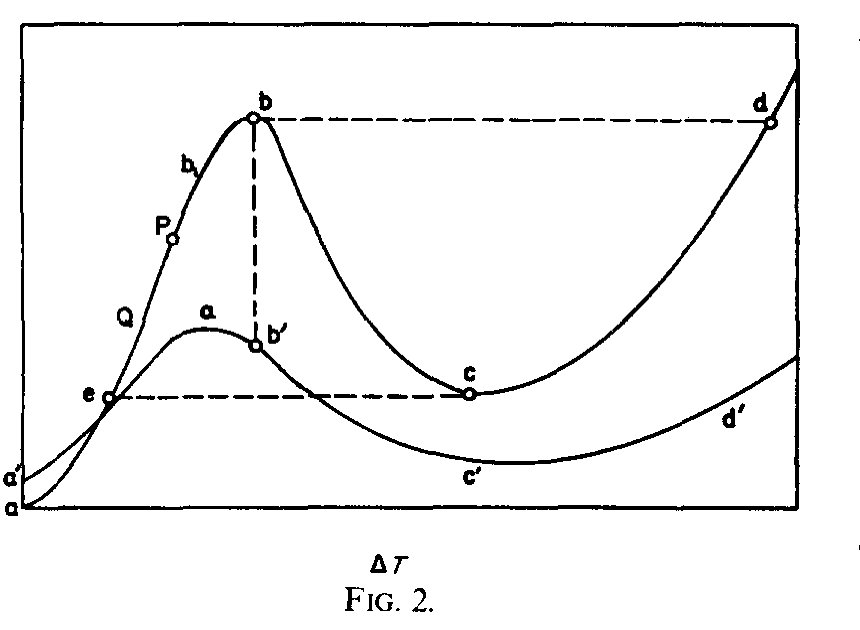
\includegraphics[width=0.95\columnwidth]{Figure/Nukiyama_Fig02_TheoryCurve.png}}
\caption{Theoretical $Q$--$\Delta T$ (upper curve, peak at $b$) and $\alpha$--$\Delta T$ (lower curve, peak at $a$) curves proposed by Nukiyama, showing the maximum heat flux ($Q_{\max}$ at $b$), minimum heat flux ($Q_{\min}$ at $c$), and the spheroidal state ($d$). Adapted from~\cite{nukiyama1966}.}
\label{fig:nukiyama_theory}
\end{figure}

Nukiyama's theoretical framework, illustrated in Fig.~\ref{fig:nukiyama_theory}, postulates that the heat transfer coefficient $\alpha$ is not a monotonically increasing function of $\Delta T$. In the mild boiling regime, bubble-induced agitation enhances heat transfer, causing both $\alpha$ and $Q$ to increase with $\Delta T$. However, as vapor generation becomes excessively vigorous, the metal surface becomes increasingly covered by a vapor film whose thermal conductivity is approximately one-twentieth that of liquid water. Consequently, $\alpha$ begins to decrease, and since $Q = \alpha\,\Delta T$, the heat flux must eventually reach a maximum value $Q_{\max}$ at a critical temperature difference. Beyond this point, further increases in $\Delta T$ cause $Q$ to decrease until a minimum value $Q_{\min}$ is reached; subsequently, radiant heat transfer becomes dominant and the curve turns upward again. The segment between $Q_{\max}$ and $Q_{\min}$ represents an unstable equilibrium that is difficult to realize experimentally; Nukiyama termed the high-temperature regime beyond this region the ``spheroidal state.''

To determine $Q_{\max}$ experimentally, Nukiyama faced the fundamental challenge that the required heat fluxes exceeded the capabilities of conventional heating apparatus for extended surfaces. He therefore devised two complementary experimental strategies. The primary approach, designated Experiment~I, employed a thin metallic wire simultaneously as the heating element and the heat transfer surface~\cite{nukiyama1966}. A platinum, nickel, or nichrome wire of diameter between $0.14~\mathrm{mm}$ and $0.575~\mathrm{mm}$ was mounted in a Pyrex glass vessel containing distilled water at saturation temperature. The wire was heated by direct current supplied through a Wheatstone bridge circuit, and its temperature was inferred from the bridge balance condition calibrated in an oil bath. This configuration was advantageous because the small wire volume minimized the required heating power, while the large surface-area-to-volume ratio facilitated high heat fluxes. For water at $100~^{\circ}\mathrm{C}$ under atmospheric pressure, Nukiyama determined that $Q_{\max}$ occurred at $\Delta T \approx 20$--$40~^{\circ}\mathrm{C}$, with $Q_{\max}$ in the range $1{,}080{,}000$--$1{,}800{,}000~\mathrm{kcal/(m^2\,h)}$ (i.e.\ approximately $1.3$--$2.1~\mathrm{MW/m^2}$), a value substantially greater than previously accepted estimates.

\begin{figure}[htbp]
\centering
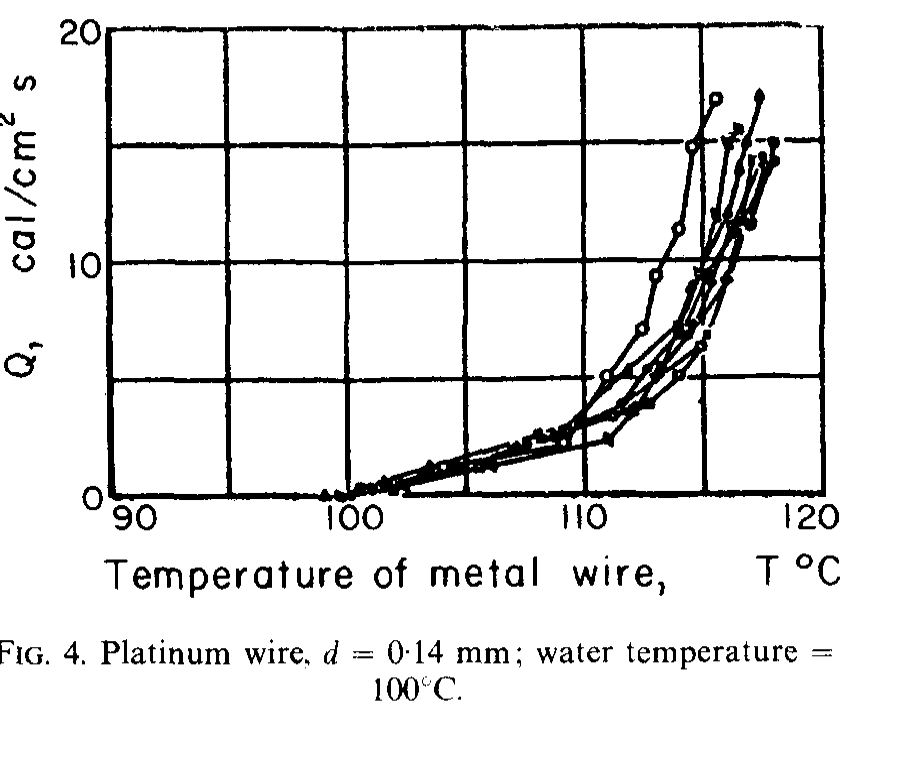
\includegraphics[width=0.92\columnwidth]{Figure/Nukiyama_Fig04_PlatinumWire.png}\\[2pt]
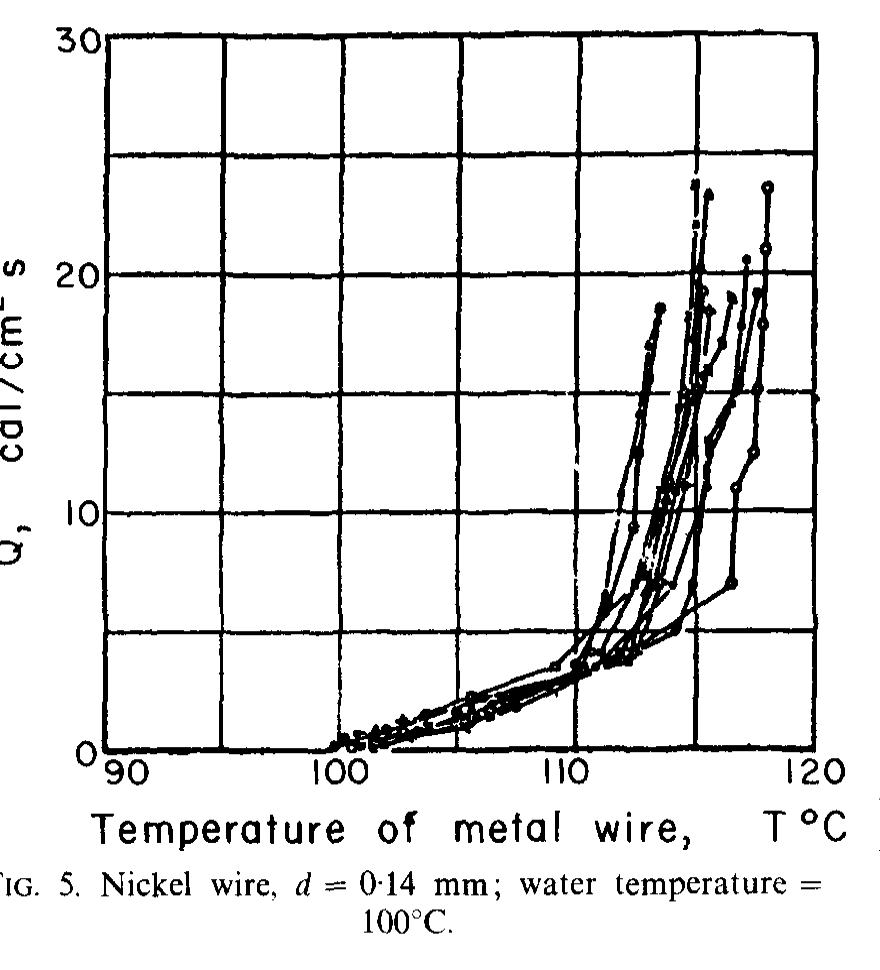
\includegraphics[width=0.92\columnwidth]{Figure/Nukiyama_Fig05_NickelWire.png}
\caption{Experimental boiling curves measured by Nukiyama for (top) a platinum wire and (bottom) a nickel wire, both of diameter $d = 0.14~\mathrm{mm}$ in water at $100~^{\circ}\mathrm{C}$. Multiple runs illustrate the considerable scatter inherent to thin-wire boiling experiments, yet the characteristic transition from natural convection to vigorous nucleate boiling near $\Delta T \approx 10$--$20~^{\circ}\mathrm{C}$ is consistently observed. Adapted from~\cite{nukiyama1966}.}
\label{fig:nukiyama_curves}
\end{figure}

The experimental boiling curves for various platinum and nickel wires, exemplified by Fig.~\ref{fig:nukiyama_curves}, exhibit considerable scatter attributable to surface contamination, electrolysis effects, and the inherent sensitivity of thin wires to minor imperfections; nevertheless, the characteristic transition from natural convection to nucleate boiling is consistently observed.

Nukiyama also conducted supplementary experiments with small circular flat plates ($10~\mathrm{mm}$ and $6.58~\mathrm{mm}$ diameter) to verify that the existence of $Q_{\max}$ was not an artifact of the wire geometry. These experiments confirmed that $Q_{\max}$ increased as the heating surface area decreased, and revealed that the flow pattern induced by bubble motion significantly influenced the maximum achievable heat flux. The comprehensive dataset and physical insights presented in Nukiyama's work established the conceptual foundation for the boiling curve that remains central to heat transfer engineering, and demonstrated that controlled experimentation with simplified geometries---such as a thin heated wire---could yield quantitative results of both scientific and practical significance.

\subsection{The Purpose of This Experiment}
Motivated by the enduring relevance of Nukiyama's findings and the practical importance of pool boiling in thermal management applications, the present study aims to replicate the essential features of the original experiment using a simplified, low-cost apparatus suitable for an advanced teaching laboratory. A test piece comprising a thin platinum wire (nominal diameter $D_w \approx 100~\mathrm{\mu m}$, length $L_w \approx 60~\mathrm{mm}$) is mounted on a pair of wooden chopsticks and immersed in demineralized water at room temperature and atmospheric pressure. Joule heating is supplied by a DC power source operating in constant-voltage mode, and the applied voltage, current, and water temperature are recorded at incremental voltage steps. From these raw measurements, the average wire temperature is inferred from the temperature-dependent electrical resistivity of platinum; subsequently, the heating power, heat flux, and convective heat transfer coefficient are computed. Crucially, the measuring uncertainties of all directly and indirectly determined quantities are propagated via the Root Sum of Square (RSS) method in order to assess the reliability of the derived boiling curve and to identify the dominant sources of experimental error. Through this exercise, we seek to verify the characteristic transition from single-phase natural convection to nucleate boiling, to quantify the associated heat transfer coefficients, and to demonstrate that a pedagogical implementation of Nukiyama's experiment can yield physically meaningful results when coupled with rigorous data postprocessing and error analysis.

% ============================================================
\section{Methodology}
% ============================================================

\subsection{Test Piece Realization}
The test piece was realized following the standardized protocol described in the laboratory manual~\cite{cioncolini2025}. A rectangular wooden block served as the base, and two chopsticks were mounted onto it using elastic rubber bands, maintaining a tip-to-tip spacing of approximately 55~mm. This configuration provides electrical insulation between the electrodes while permitting easy adjustment of their alignment and separation.

\begin{figure}[htbp]
\centerline{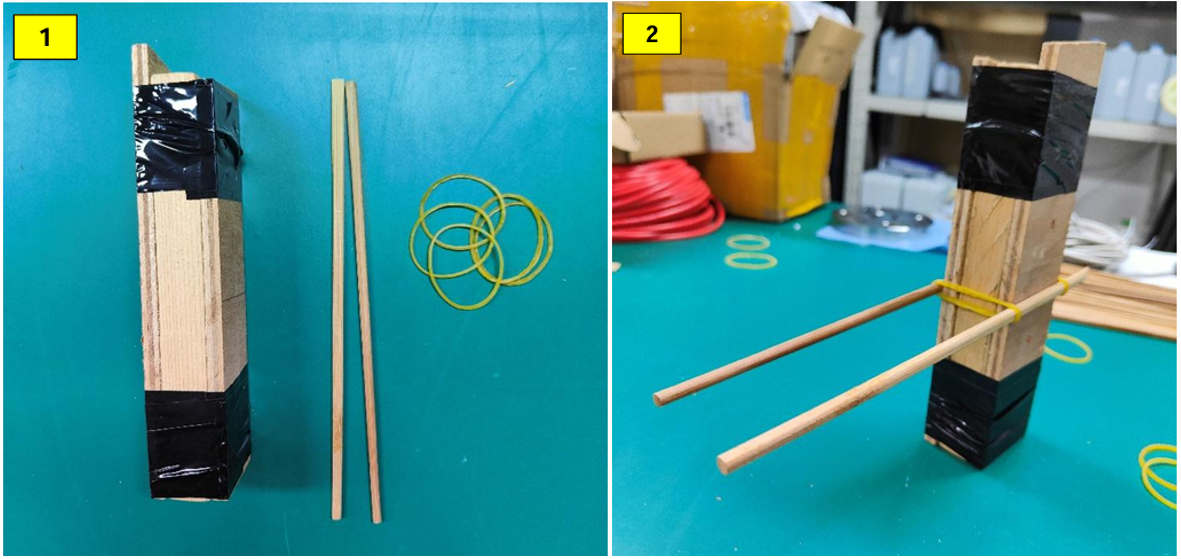
\includegraphics[width=0.95\columnwidth]{Figure/Method_Fig06_BaseLayout.png}}
\caption{Base layout of the test piece assembly.}
\label{fig:base_layout}
\end{figure}

Two strips of aluminum foil (20~mm~$\times$~30~mm) were wrapped around the tips of the chopsticks and secured with adhesive paper tape, leaving a portion of the foil exposed to establish the electrical contact area. A platinum wire segment approximately 10--15~cm in length was then wound around the exposed foil at each electrode tip and fixed with adhesive tape applied to the rear face of the chopsticks.

\begin{figure}[htbp]
\centerline{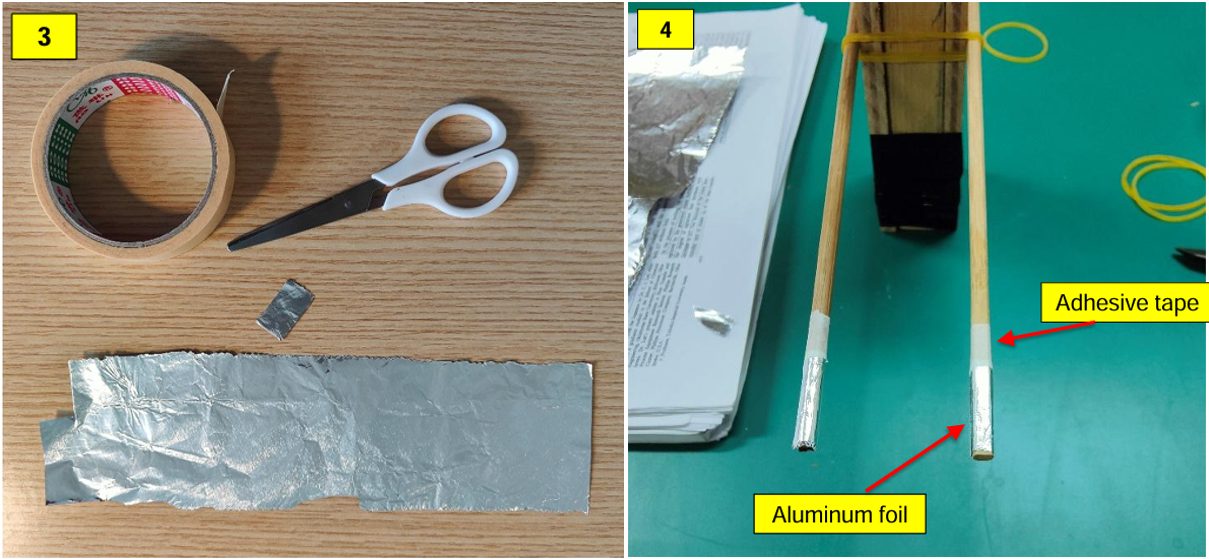
\includegraphics[width=0.95\columnwidth]{Figure/Method_Fig07_Electrode.png}}
\caption{Electrode substrate fabrication with aluminum foil contact areas.}
\label{fig:electrode}
\end{figure}

The leads from the DC power supply were routed to the test piece with one cable terminal initially left disconnected as a safety precaution against hazardous current flow during assembly. The cables were clamped to the chopsticks so that the stripped conductor rested on the aluminum foil electrodes. Two cable ties were fastened on each chopstick---one on either side of the platinum wire---to secure the stripped cable sections firmly against the electrodes; excess tails were trimmed upon tightening.

\begin{figure}[htbp]
\centerline{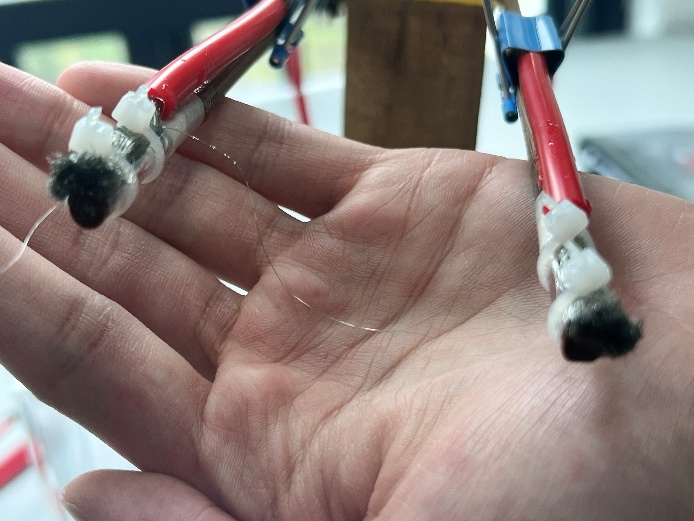
\includegraphics[width=0.75\columnwidth]{Figure/Method_Fig08_WireFixation.jpeg}}
\caption{Platinum wire and cable fixation on the chopstick electrodes.}
\label{fig:wire_fixation}
\end{figure}

To ensure a straight, sag-free wire span, mechanical tension was applied by inserting a small piece of carton board beneath the chopstick assembly. A multimeter was then used to check electrical continuity between the two electrodes and to measure the approximate resistance of the platinum wire, providing a baseline value for later verification against the DC power supply readings.

\begin{figure}[htbp]
\centerline{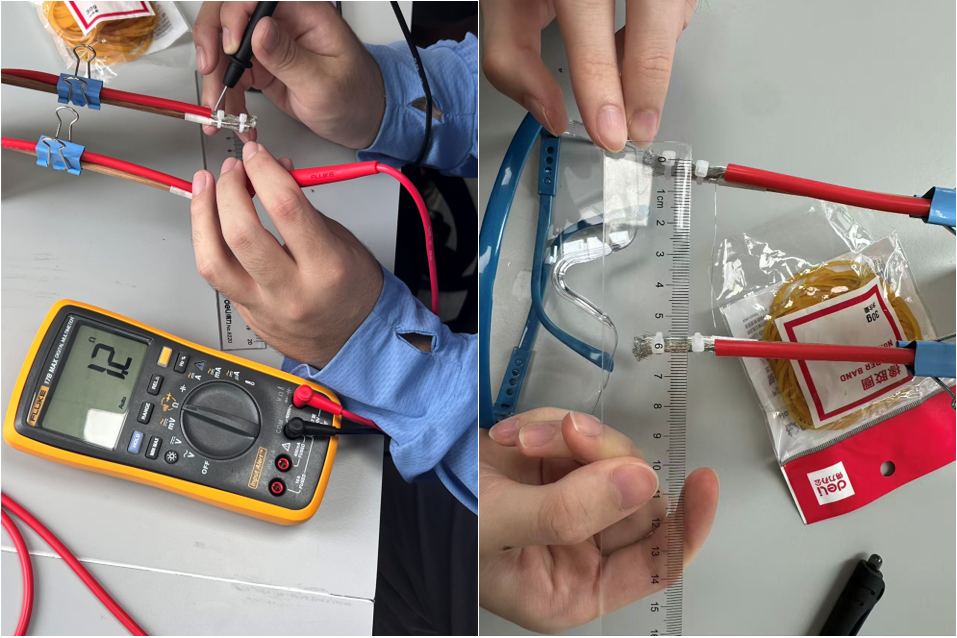
\includegraphics[width=0.95\columnwidth]{Figure/Method_Fig09_Continuity.png}}
\caption{Verification of electrical continuity and measurement of the platinum wire resistance and active length~$L_w$.}
\label{fig:continuity}
\end{figure}

Finally, the platinum wire was cleaned with an ear bud soaked in isopropyl alcohol to remove skin oils and grease deposited during handling. The active wire length $L_w$ was measured with a ruler and recorded for subsequent calculations.

\subsection{Experimental Setup}
The experimental setup was assembled following the standardized procedure outlined in the laboratory manual~\cite{cioncolini2025}. The test piece was positioned on top of the transparent water tank, maintaining a clearance of approximately 30--40~mm from the bottom surface to allow unrestricted bubble motion and natural convection currents. The probe of the water temperature sensor was immersed in the tank and secured with a clamp to prevent displacement during the experiment.

\begin{figure}[htbp]
\centerline{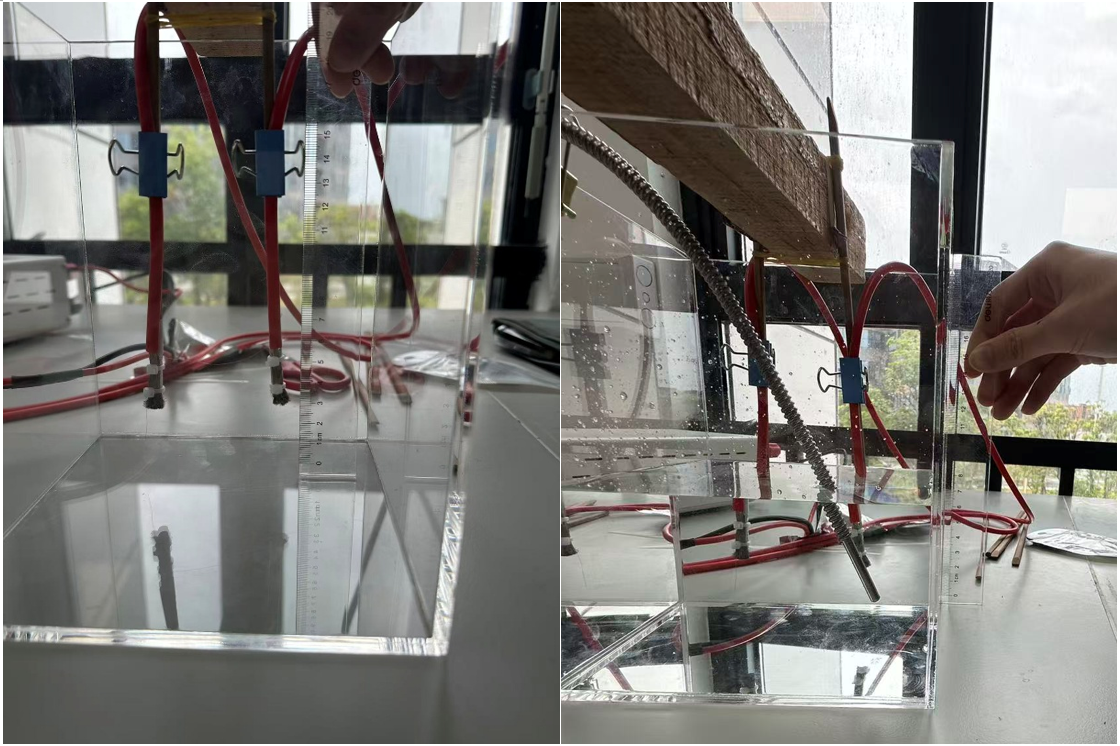
\includegraphics[width=0.95\columnwidth]{Figure/Method_Fig10_Setup.png}}
\caption{Measurement of the electrode position and water submersion depth.}
\label{fig:setup}
\end{figure}

The tank was filled with demineralized water until the platinum wire was submerged by approximately 20--30~mm, ensuring adequate heat transfer area while minimizing hydrostatic pressure effects. Prior to energizing the circuit, the DC power supply was switched on and configured to operate in constant-voltage (C.V.) mode; the output was manually zeroed to prevent an uncontrolled inrush of current upon connection. The previously disconnected positive cable terminal was then secured to the power supply output, completing the electrical circuit for the subsequent experimental procedure.

\subsection{Experiment Execution and Data Recording}
The experimental procedure was conducted in accordance with the protocol described in the course materials~\cite{cioncolini2025}. With the DC power supply operating in constant-voltage mode and the circuit fully connected, the voltage control knob was adjusted to deliver an initial potential difference of 1.0~V across the platinum wire. The system was allowed to stabilize for several seconds until the readings of the integrated voltmeter and ammeter, as well as the water temperature indicated by the temperature sensor, exhibited no appreciable transient drift.

\begin{figure}[htbp]
\centerline{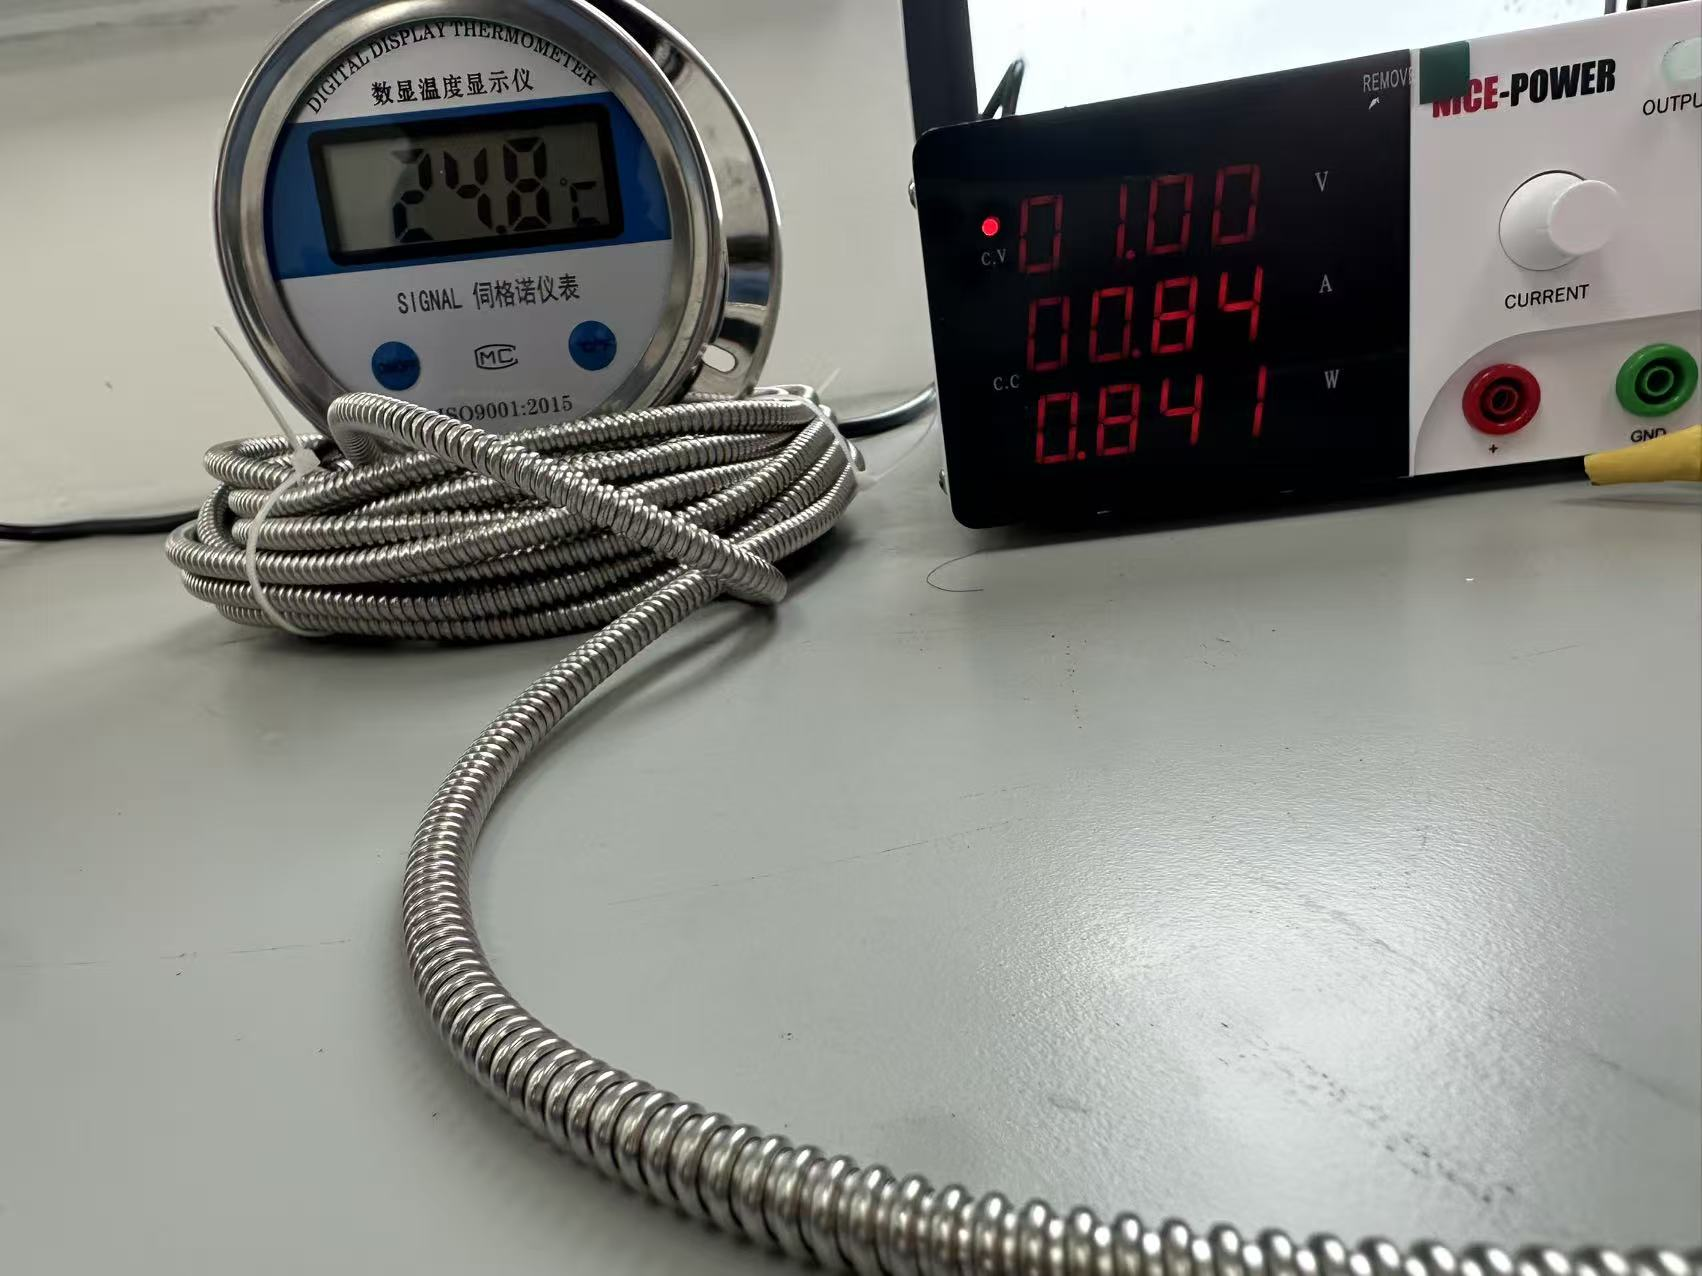
\includegraphics[width=\columnwidth]{Figure/Method_Fig11_TempSensor.jpeg}}
\caption{Temperature sensor and DC power supply at the initial operating condition of 1~V.}
\label{fig:temp_sensor}
\end{figure}

Once a quasi-steady state was attained, the voltage $V$ across the wire, the current $I$ flowing through it, and the bulk water temperature $T_{\mathrm{water}}$ were recorded. The voltage was then incremented in steps of 0.2~V (i.e., 1.2~V, 1.4~V, 1.6~V, and so forth), and the measurement sequence was repeated at each level. This progressive increase was continued until the terminal voltage reached approximately 8--9~V, yielding a total of 30--40 data points spanning the transition from single-phase natural convection to fully developed nucleate boiling. Throughout the tests, the measured values were entered into a spreadsheet template in real time to monitor the emerging boiling curve and to identify any anomalous behavior.

\subsection{Data Reduction}
From each raw triplet $(V,I,T_{\mathrm{water}})$ the following derived quantities were computed. The instantaneous electrical resistivity of the platinum wire is
\begin{equation}
\rho \;=\; \frac{R\,A}{L_w} \;=\; \frac{\pi D_w^{2}}{4 L_w}\cdot\frac{V}{I},
\label{eq:rho}
\end{equation}
where $A = \pi D_w^2/4$ is the cross-sectional area and $R = V/I$ is the wire resistance. Treating platinum's resistivity as a linear function of temperature in the relevant range,
\begin{equation}
\rho(T) \;=\; \rho_{0} + \alpha\,T,
\label{eq:rhoT}
\end{equation}
with $\rho_{0} = 9.847\times10^{-8}~\Omega\,\mathrm{m}$ and $\alpha = 3.744\times10^{-10}~\Omega\,\mathrm{m}/^{\circ}\mathrm{C}$, the spatially averaged wire temperature is
\begin{equation}
T_{\mathrm{wire}} \;=\; \frac{\rho - \rho_{0}}{\alpha}.
\label{eq:Twire}
\end{equation}
The Joule heating power dissipated in the wire is
\begin{equation}
W \;=\; V\,I,
\label{eq:W}
\end{equation}
and, assuming that the wire surface acts as the sole heat transfer surface, the surface-averaged heat flux is
\begin{equation}
q'' \;=\; \frac{W}{\pi D_w L_w}.
\label{eq:flux}
\end{equation}
Finally, the convective heat transfer coefficient relative to the bulk water is
\begin{equation}
h \;=\; \frac{q''}{T_{\mathrm{wire}} - T_{\mathrm{water}}}.
\label{eq:HTC}
\end{equation}

\subsection{Uncertainty Propagation}
Each derived quantity inherits the random uncertainty of the underlying measurements. Assuming uncorrelated, normally distributed input errors, the standard combination rule (Root Sum of Square, RSS) yields, for any indirectly determined quantity $y = f(x_1,\ldots,x_n)$,
\begin{equation}
\delta y \;=\; \sqrt{\sum_{i=1}^{n}\!\left(\frac{\partial f}{\partial x_i}\,\delta x_i\right)^{2}}.
\label{eq:RSS}
\end{equation}
Application of \eqref{eq:RSS} to \eqref{eq:rho}--\eqref{eq:HTC}, taking advantage of the fact that all relationships are products or quotients of measured quantities, gives the following relative uncertainties:
\begin{align}
\frac{\delta\rho}{\rho} &= \sqrt{4\!\left(\tfrac{\delta D_w}{D_w}\right)^{2}+\!\left(\tfrac{\delta L_w}{L_w}\right)^{2}+\!\left(\tfrac{\delta V}{V}\right)^{2}+\!\left(\tfrac{\delta I}{I}\right)^{2}},\\
\delta T_{\mathrm{wire}} &= \frac{\delta\rho}{\alpha},\\
\frac{\delta W}{W} &= \sqrt{\!\left(\tfrac{\delta V}{V}\right)^{2}+\!\left(\tfrac{\delta I}{I}\right)^{2}},\\
\frac{\delta q''}{q''} &= \sqrt{\!\left(\tfrac{\delta W}{W}\right)^{2}+\!\left(\tfrac{\delta D_w}{D_w}\right)^{2}+\!\left(\tfrac{\delta L_w}{L_w}\right)^{2}},\\
\frac{\delta h}{h} &= \sqrt{\!\left(\tfrac{\delta q''}{q''}\right)^{2}+\frac{\delta T_{\mathrm{wire}}^{2}+\delta T_{\mathrm{water}}^{2}}{\left(T_{\mathrm{wire}}-T_{\mathrm{water}}\right)^{2}}}.
\end{align}
Note that the factor of $4$ in the expression for $\delta\rho/\rho$ originates from the quadratic dependence of cross-sectional area on diameter, $A \propto D_w^{2}$, which makes the wire diameter an especially sensitive input. The propagated uncertainties were evaluated point-by-point for every operating condition and are reported throughout Sections~\ref{sec:dp} and~\ref{sec:results} as error bars and percentage bands.

% ============================================================
\section{Data Processing}
\label{sec:dp}
% ============================================================

This section traces the chain of derived quantities introduced in the Methodology, beginning with the raw electrical measurements and culminating in the derived heat transfer parameters. At each step the corresponding uncertainty contribution is examined, identifying which inputs dominate the overall error budget.

\subsection{Raw Measurements}
Figs.~\ref{fig:fig01}--\ref{fig:fig03} display the recorded voltage, current, and water temperature as a function of the data-point index. The voltage was ramped monotonically from $1.0~\mathrm{V}$ to $8.4~\mathrm{V}$ in nominally uniform increments, but the current exhibited a clearly sublinear response: as the wire heated up, its resistance increased due to the positive temperature coefficient of platinum, so $I$ grew more slowly than $V$. The water temperature drifted only modestly between $24.8~^{\circ}\mathrm{C}$ and $25.2~^{\circ}\mathrm{C}$ throughout the test, confirming that the bulk pool remained essentially at room temperature and that the experiment is performed under strongly subcooled conditions rather than at saturation.

\begin{figure}[htbp]
\centerline{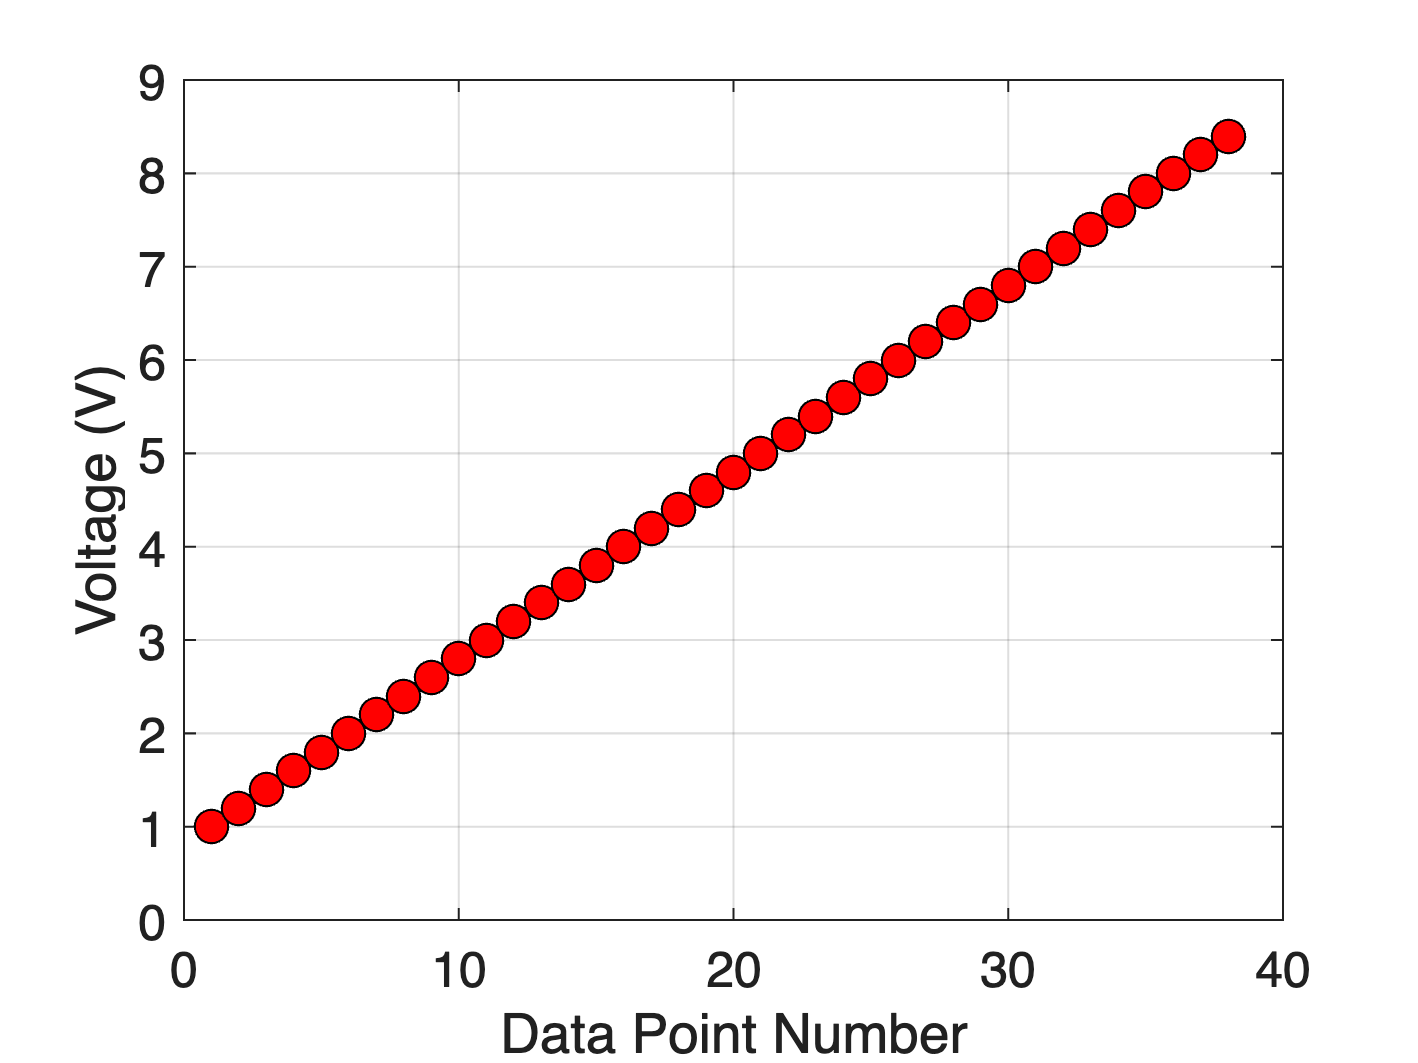
\includegraphics[width=\columnwidth]{Figure/Fig01_Voltage.png}}
\caption{Applied voltage $V$ versus data-point index. The voltage was incremented in approximately uniform $0.2~\mathrm{V}$ steps from $1.0~\mathrm{V}$ to $8.4~\mathrm{V}$.}
\label{fig:fig01}
\end{figure}

\begin{figure}[htbp]
\centerline{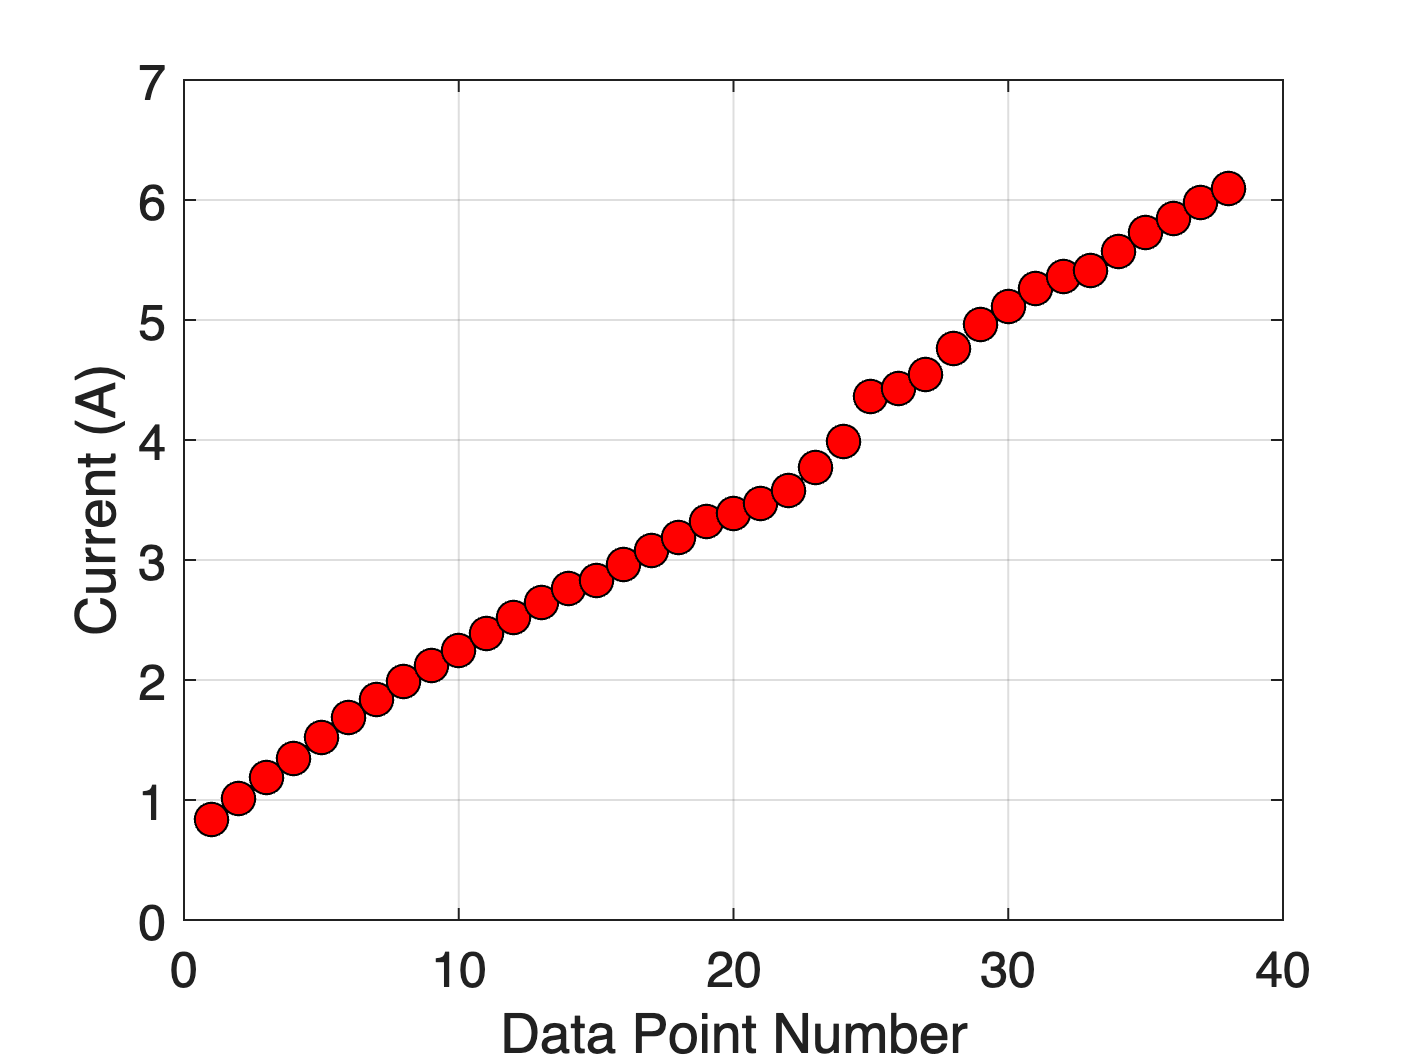
\includegraphics[width=\columnwidth]{Figure/Fig02_Current.png}}
\caption{Measured current $I$ versus data-point index. The sublinear growth of $I$ relative to $V$ reflects the temperature-induced increase of the wire resistance.}
\label{fig:fig02}
\end{figure}

\begin{figure}[htbp]
\centerline{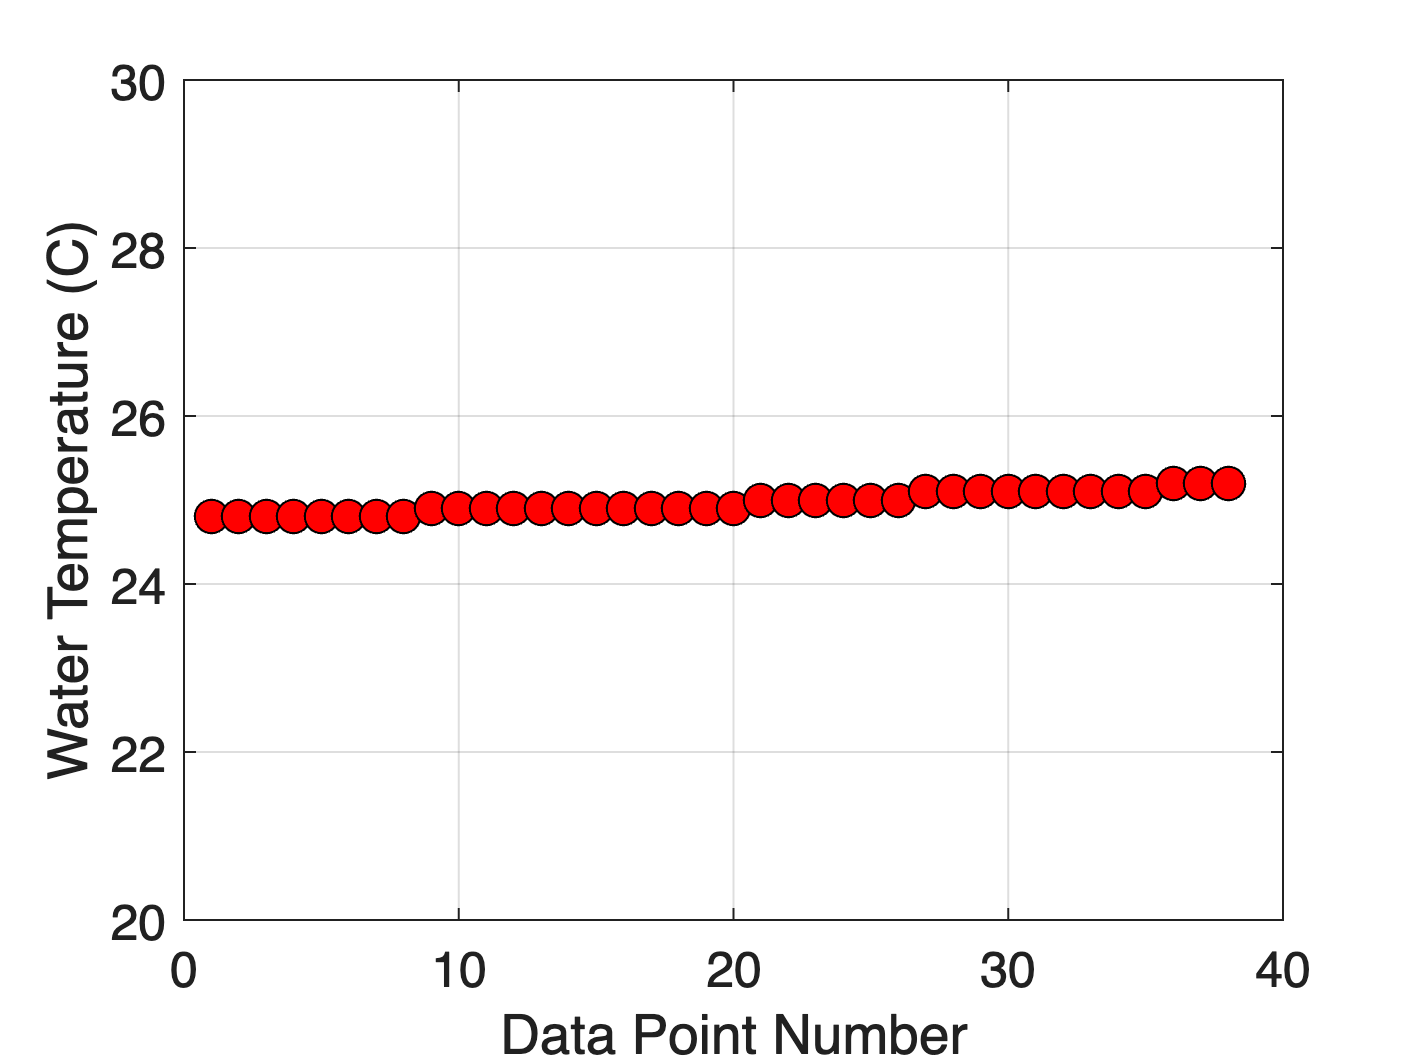
\includegraphics[width=\columnwidth]{Figure/Fig03_WaterTemperature.png}}
\caption{Bulk water temperature $T_{\mathrm{water}}$ versus data-point index. The pool remained at $\approx 25~^{\circ}\mathrm{C}$, indicating strongly subcooled boiling conditions.}
\label{fig:fig03}
\end{figure}

\subsection{Uncertainty of the Raw Inputs}
Equations~\eqref{eq:delV}--\eqref{eq:delI} translate the multimeter accuracy specification into absolute uncertainties whose relative contribution is large at low readings and small at high readings. Figs.~\ref{fig:fig04}--\ref{fig:fig05} plot the resulting percentage uncertainty in $V$ and $I$ as a function of the reading. At the lowest voltage step ($V=1~\mathrm{V}$, $I\approx 0.84~\mathrm{A}$) both uncertainties exceed $2\%$, whereas at the largest reading ($V=8.4~\mathrm{V}$, $I\approx 6.1~\mathrm{A}$) they fall below $1.2\%$. Consequently, the early low-power points carry disproportionately larger random errors than the high-power points, an effect that will reappear when the propagated uncertainty of derived quantities is examined.

\begin{figure}[htbp]
\centerline{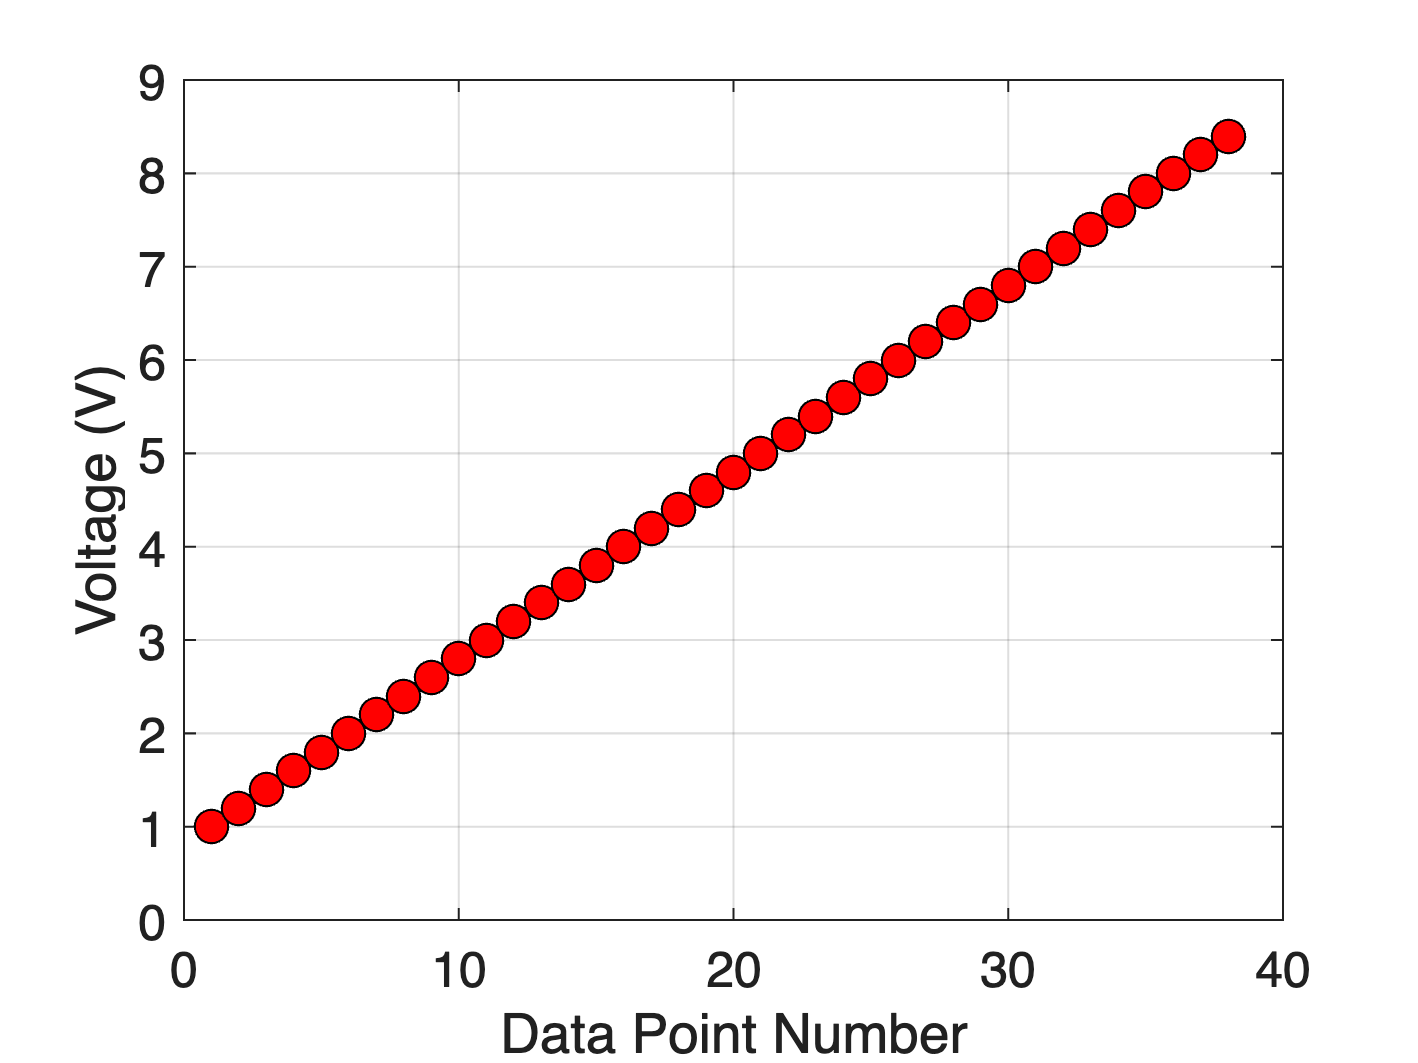
\includegraphics[width=\columnwidth]{Figure/Fig01_Voltage.png}}
\caption{Relative uncertainty of the applied voltage, $\delta V/V$, as a function of $V$.}
\label{fig:fig04}
\end{figure}

\begin{figure}[htbp]
\centerline{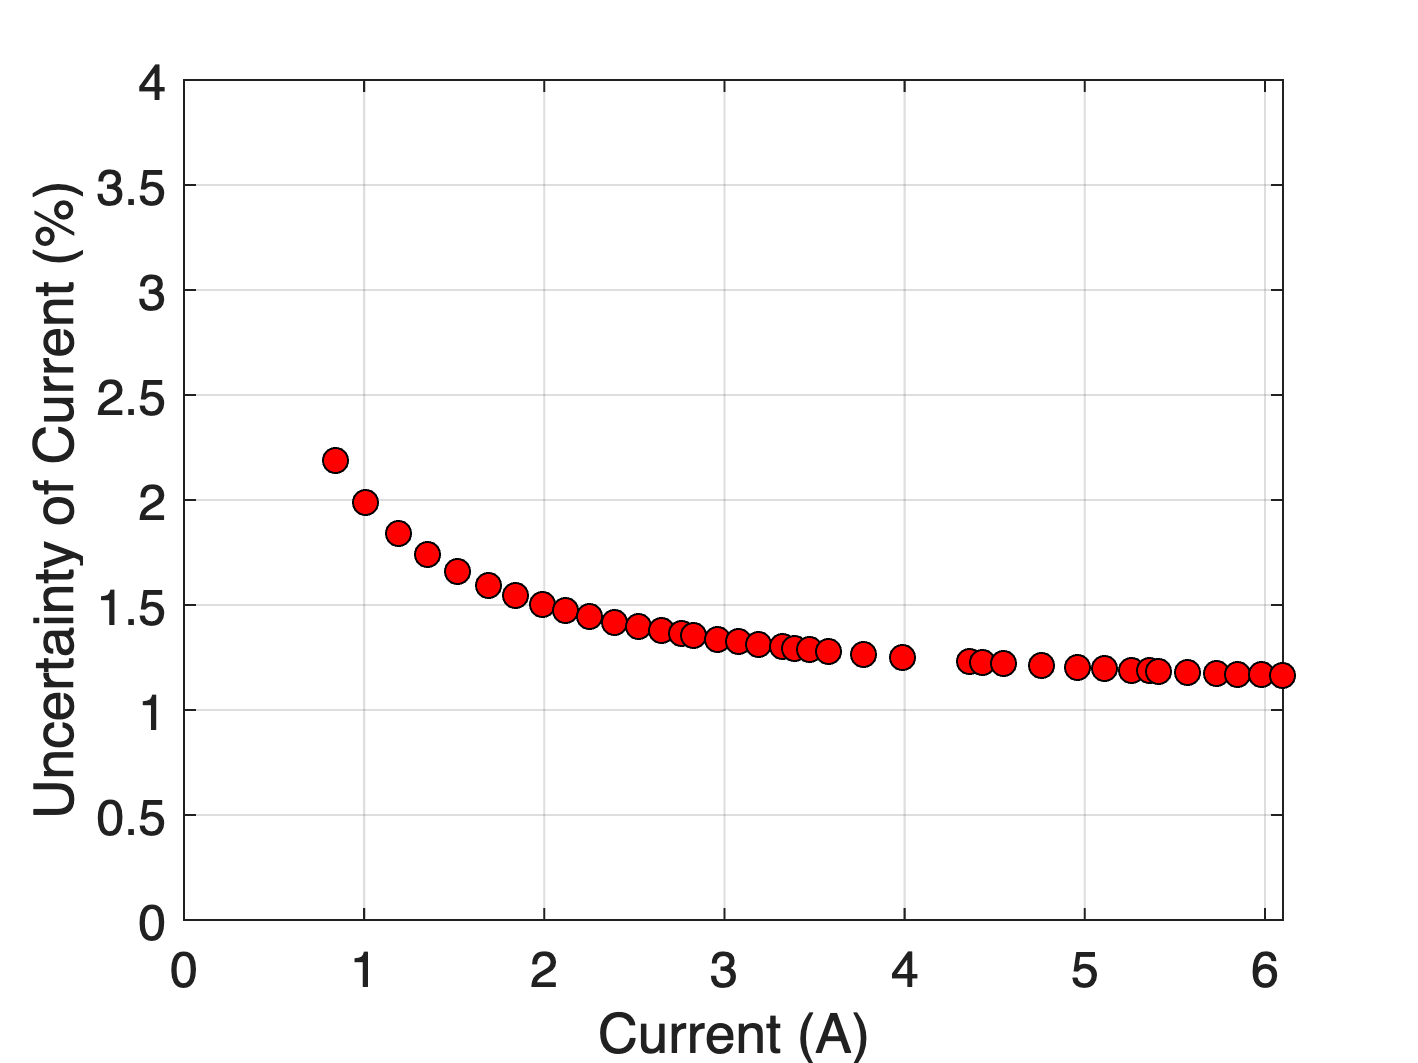
\includegraphics[width=\columnwidth]{Figure/Fig05_CurrentUncertainty.png}}
\caption{Relative uncertainty of the measured current, $\delta I/I$, as a function of $I$.}
\label{fig:fig05}
\end{figure}

\subsection{Resistivity and Wire Temperature}
Application of \eqref{eq:rho} to every measurement yields the resistivity sequence whose relative uncertainty is shown in Fig.~\ref{fig:fig06}. Because $\delta\rho/\rho$ combines the propagated $V$ and $I$ uncertainties with the geometric tolerances of the wire, it falls in the range $2$--$4\%$ across the dataset, dominated by $\delta D_w/D_w$ at high readings (since $\delta V/V$ and $\delta I/I$ become small) and by $\delta V/V$, $\delta I/I$ at low readings.

Conversion of $\rho$ to wire temperature through \eqref{eq:Twire} amplifies these errors considerably: $\delta T_{\mathrm{wire}} = \delta\rho/\alpha$, and the small numerical value of $\alpha = 3.744\times10^{-10}~\Omega\,\mathrm{m}/^{\circ}\mathrm{C}$ means that a $1\%$ uncertainty in $\rho$---corresponding to roughly $1.6\times10^{-9}~\Omega\,\mathrm{m}$ at typical operating points---propagates to about $4~^{\circ}\mathrm{C}$ in $T_{\mathrm{wire}}$. Figs.~\ref{fig:fig07}--\ref{fig:fig08} present this propagated uncertainty in both percentage and absolute forms. The absolute uncertainty in wire temperature reaches $15$--$20~^{\circ}\mathrm{C}$ at high heat fluxes, while the percentage uncertainty remains below $10\%$ because the wire temperature itself is large ($150$--$245~^{\circ}\mathrm{C}$). The shallow slope of platinum's resistivity--temperature relationship is therefore the principal limitation of the resistance thermometry technique employed here.

\begin{figure}[htbp]
\centerline{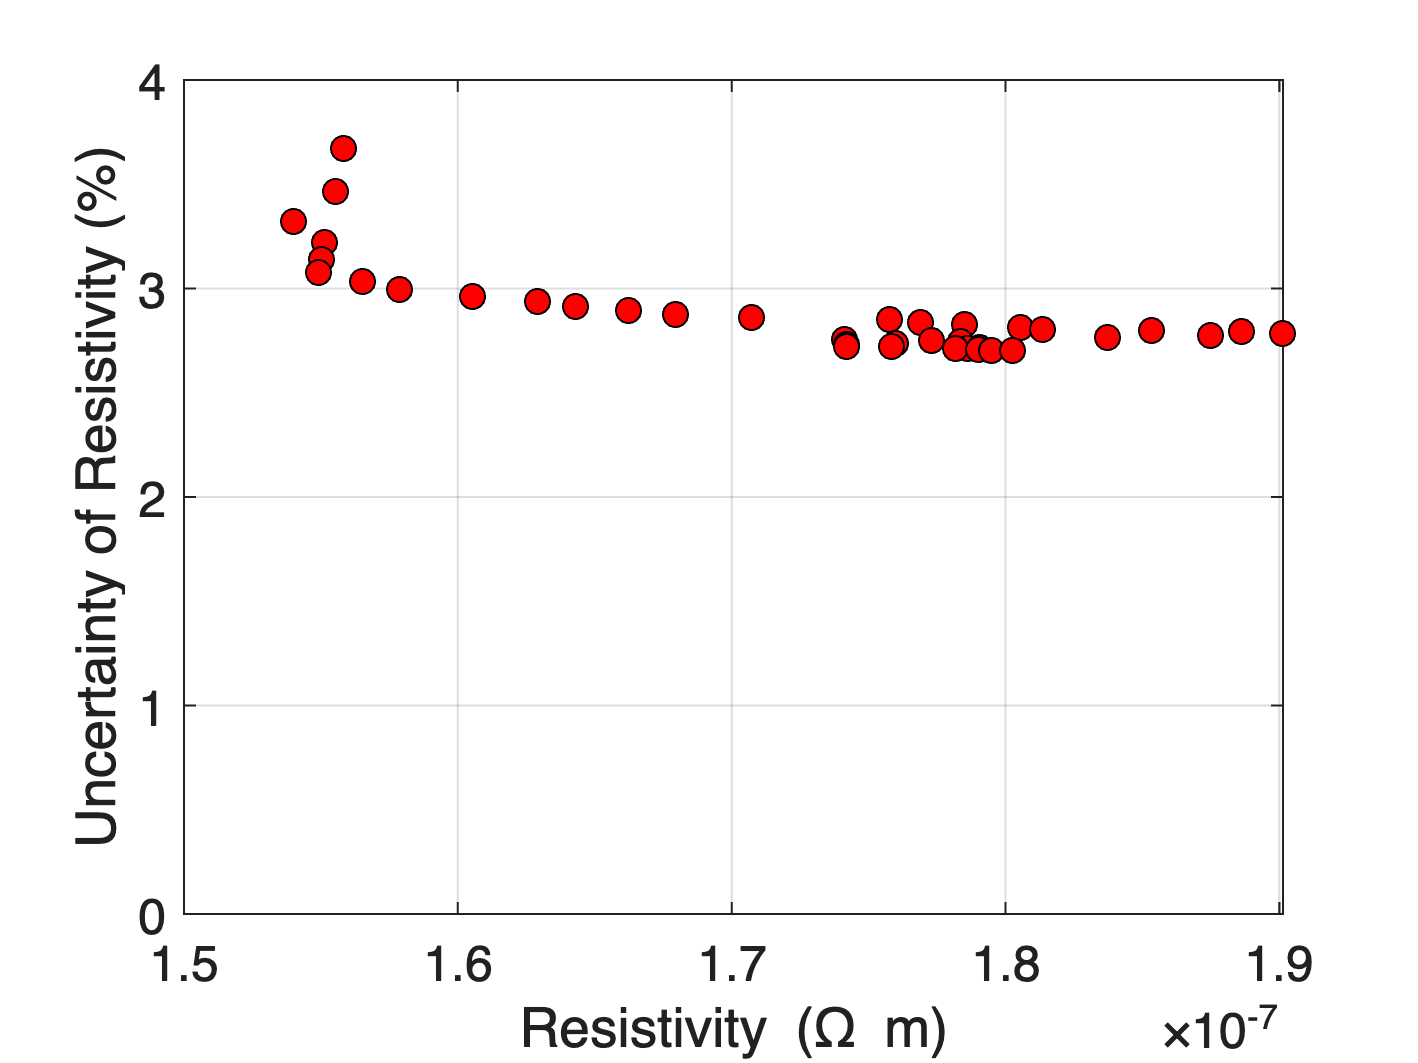
\includegraphics[width=\columnwidth]{Figure/Fig06_ResistivityUncertainty.png}}
\caption{Relative uncertainty of the wire resistivity, $\delta\rho/\rho$.}
\label{fig:fig06}
\end{figure}

\begin{figure}[htbp]
\centerline{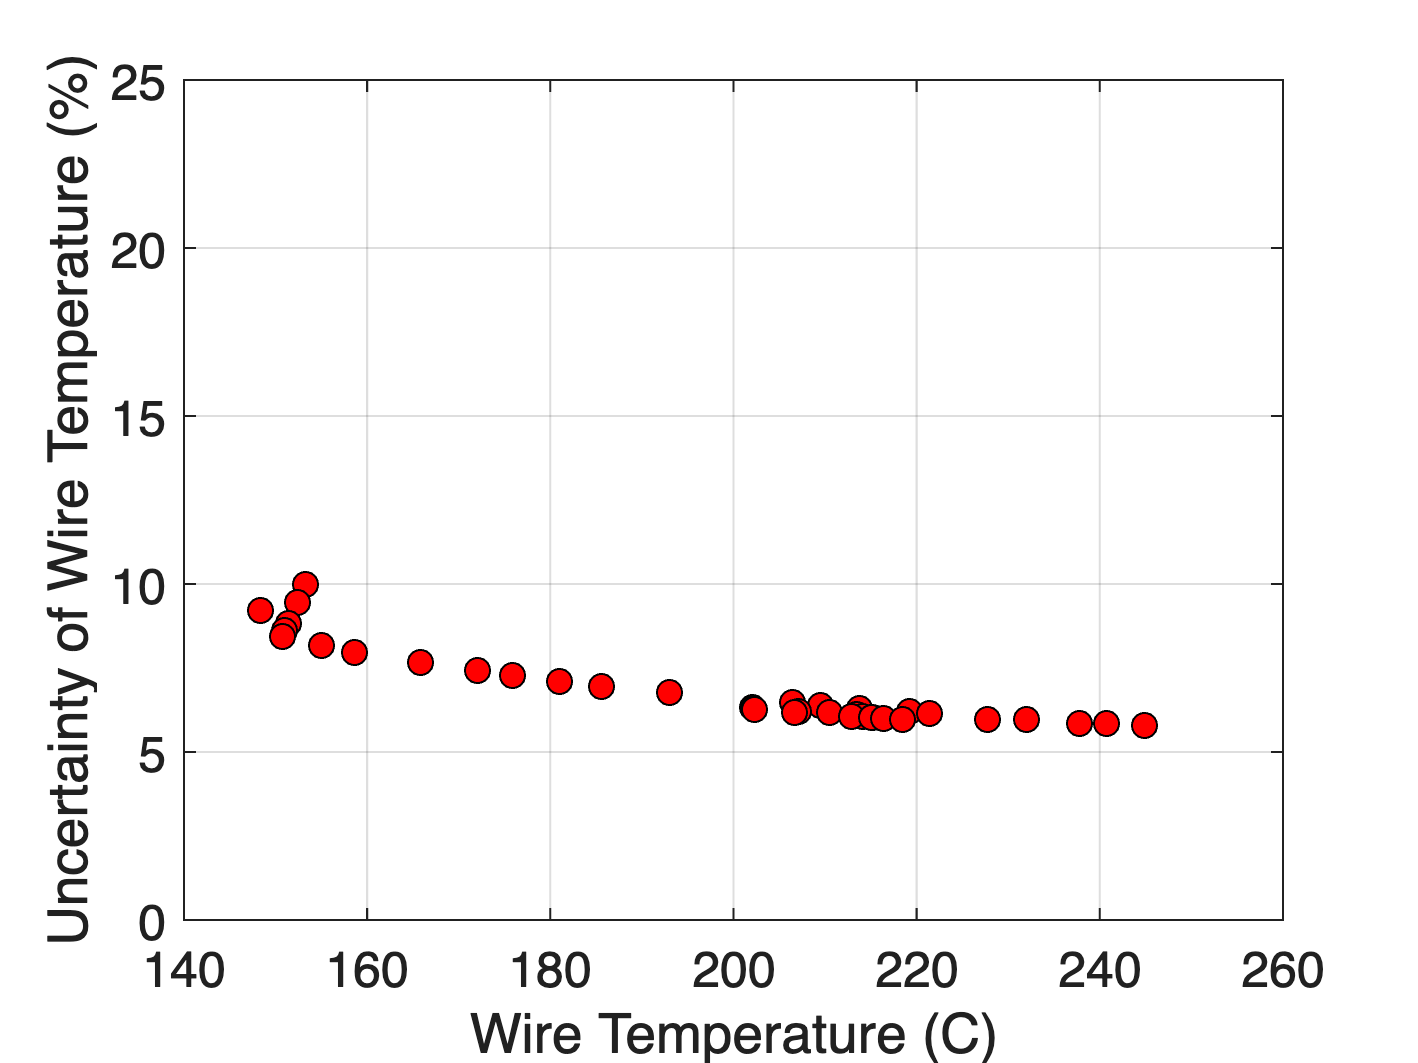
\includegraphics[width=\columnwidth]{Figure/Fig07_WireTempUncertaintyPct.png}}
\caption{Percentage uncertainty of the inferred wire temperature, $\delta T_{\mathrm{wire}}/T_{\mathrm{wire}}$.}
\label{fig:fig07}
\end{figure}

\begin{figure}[htbp]
\centerline{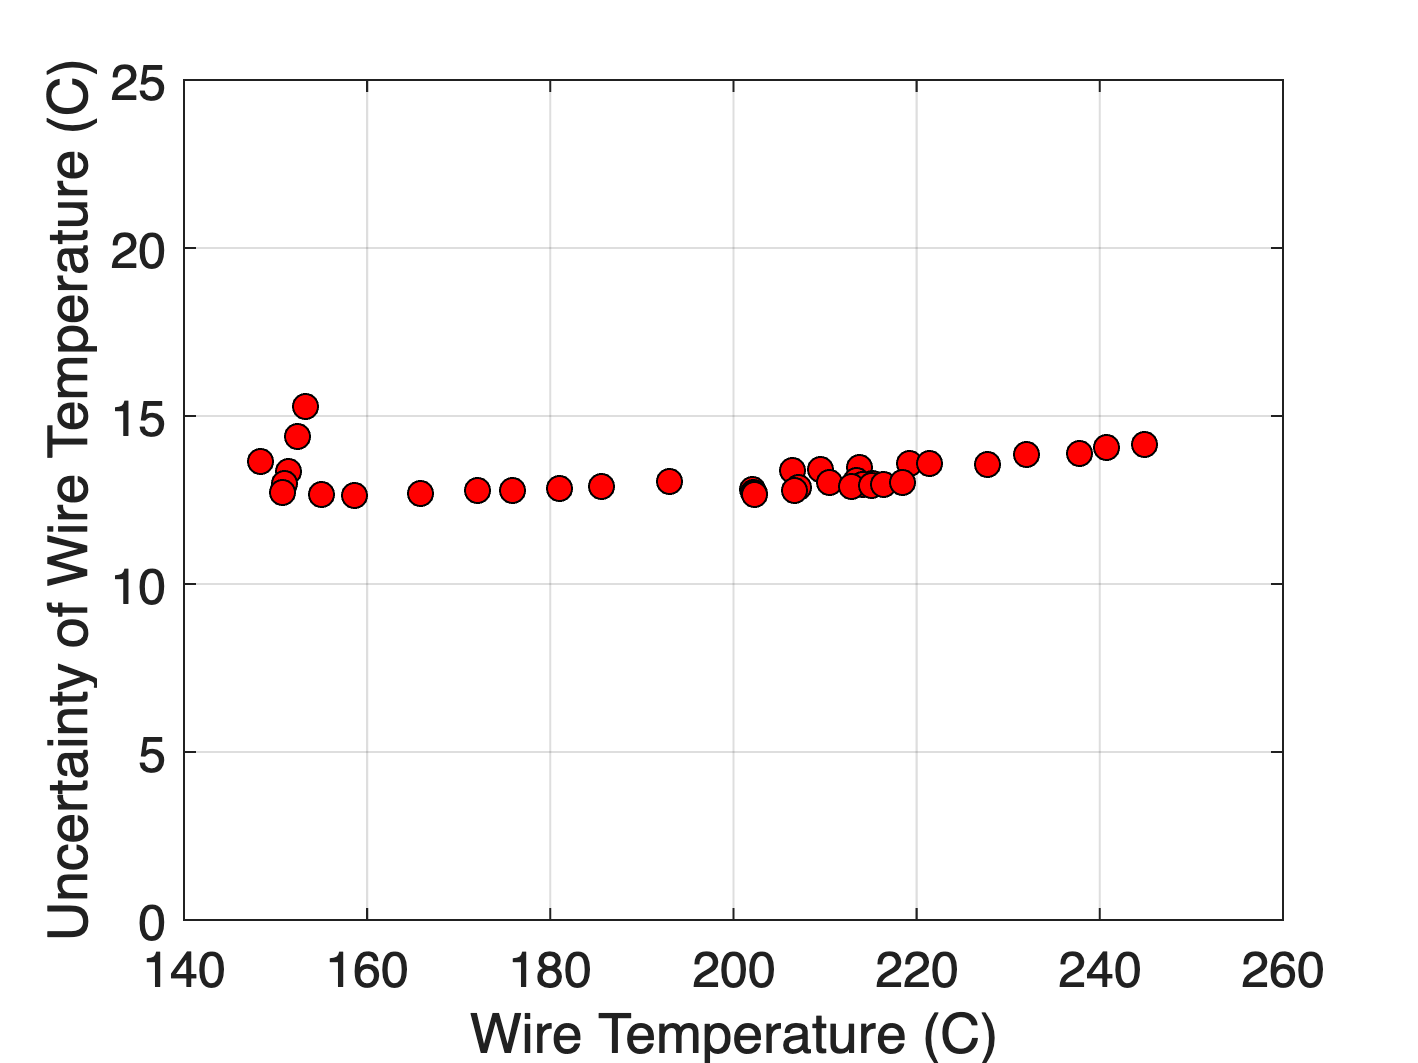
\includegraphics[width=\columnwidth]{Figure/Fig08_WireTempUncertaintyAbs.png}}
\caption{Absolute uncertainty of the wire temperature, $\delta T_{\mathrm{wire}}$ in $^{\circ}\mathrm{C}$, plotted against $T_{\mathrm{wire}}$.}
\label{fig:fig08}
\end{figure}

Fig.~\ref{fig:fig09} compares the inferred wire temperature with the simultaneously recorded water temperature. The wire is several hundred degrees hotter than the surrounding pool throughout the experiment, with $T_{\mathrm{wire}}$ first climbing from $\sim 150~^{\circ}\mathrm{C}$ to a local maximum near $244~^{\circ}\mathrm{C}$ around point~22 before retreating to approximately $200$--$220~^{\circ}\mathrm{C}$ for the remainder of the test. This non-monotonic behavior, despite a monotonic voltage ramp, is the first hint of a regime change at the wire surface and will be discussed in detail in Section~\ref{sec:results}.

\begin{figure}[htbp]
\centerline{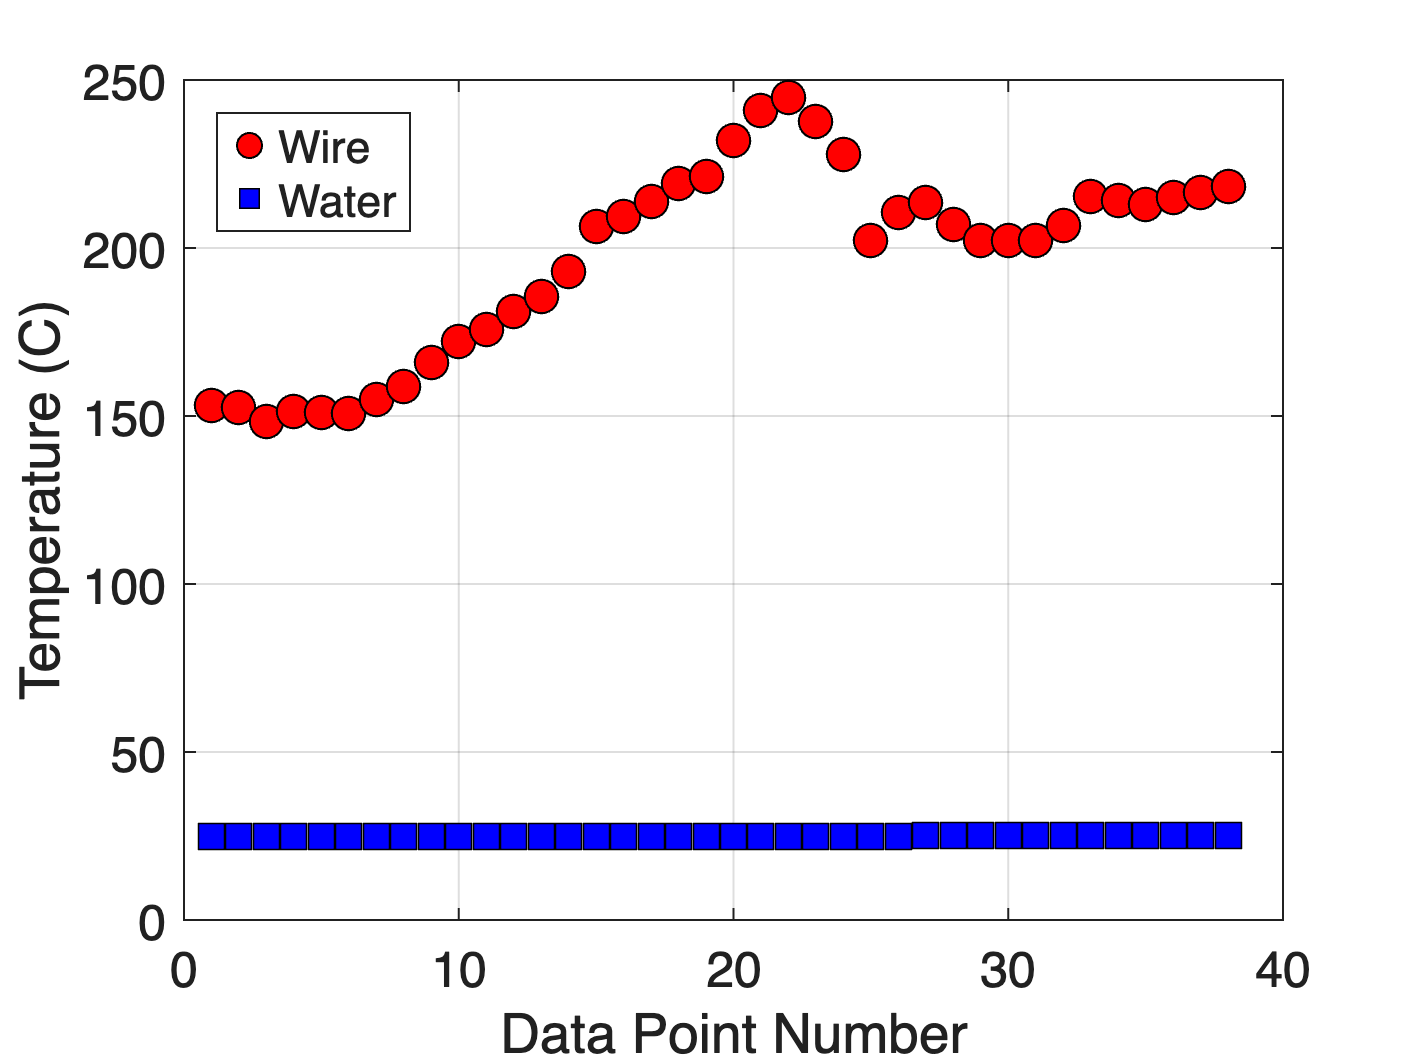
\includegraphics[width=\columnwidth]{Figure/Fig09_WireWaterTemperature.png}}
\caption{Wire temperature (red circles) and water temperature (blue squares) versus data-point index. The non-monotonic evolution of $T_{\mathrm{wire}}$ for a monotonic voltage ramp signals a boiling regime transition.}
\label{fig:fig09}
\end{figure}

\subsection{Power, Heat Flux, and Heat Transfer Coefficient}
The heating power $W = VI$ rises smoothly from less than $1~\mathrm{W}$ to slightly above $51~\mathrm{W}$ across the dataset, with the relative uncertainty $\delta W/W$ (Fig.~\ref{fig:fig10}) almost everywhere below $2\%$ and below $1.5\%$ once the readings exceed $\sim 3~\mathrm{V}$. The heat flux $q''$ (Fig.~\ref{fig:fig11}) ranges from approximately $40~\mathrm{kW/m^2}$ at the first point to over $2.7~\mathrm{MW/m^2}$ at the highest power input, with $\delta q''/q''$ slightly larger than $\delta W/W$ owing to the additional contribution of the geometric tolerances. The HTC uncertainty (Fig.~\ref{fig:fig12}) is markedly larger and exhibits a pronounced dependence on $h$ itself: at the lowest HTC values it can exceed $20\%$, whereas at the highest values it stabilizes below $10\%$. The reason is that $\delta h/h$ contains a contribution $\sim \sqrt{\delta T_{\mathrm{wire}}^{2}+\delta T_{\mathrm{water}}^{2}}/(T_{\mathrm{wire}}-T_{\mathrm{water}})$, which is amplified precisely where $\Delta T$ is small.

\begin{figure}[htbp]
\centerline{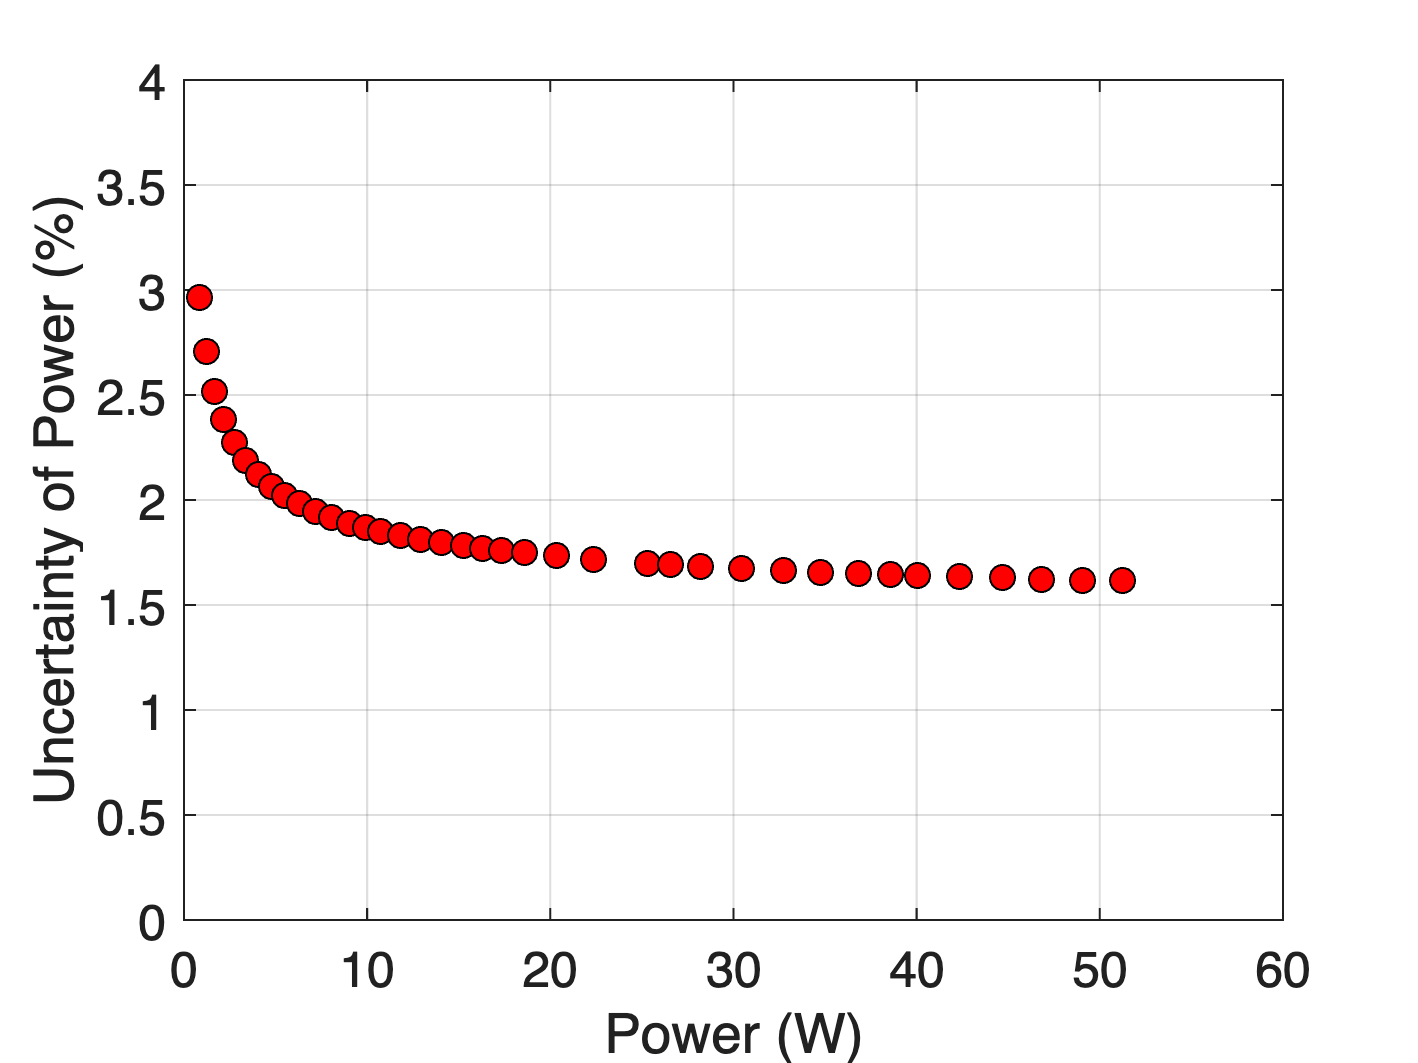
\includegraphics[width=\columnwidth]{Figure/Fig10_PowerUncertainty.png}}
\caption{Relative uncertainty of the heating power, $\delta W/W$.}
\label{fig:fig10}
\end{figure}

\begin{figure}[htbp]
\centerline{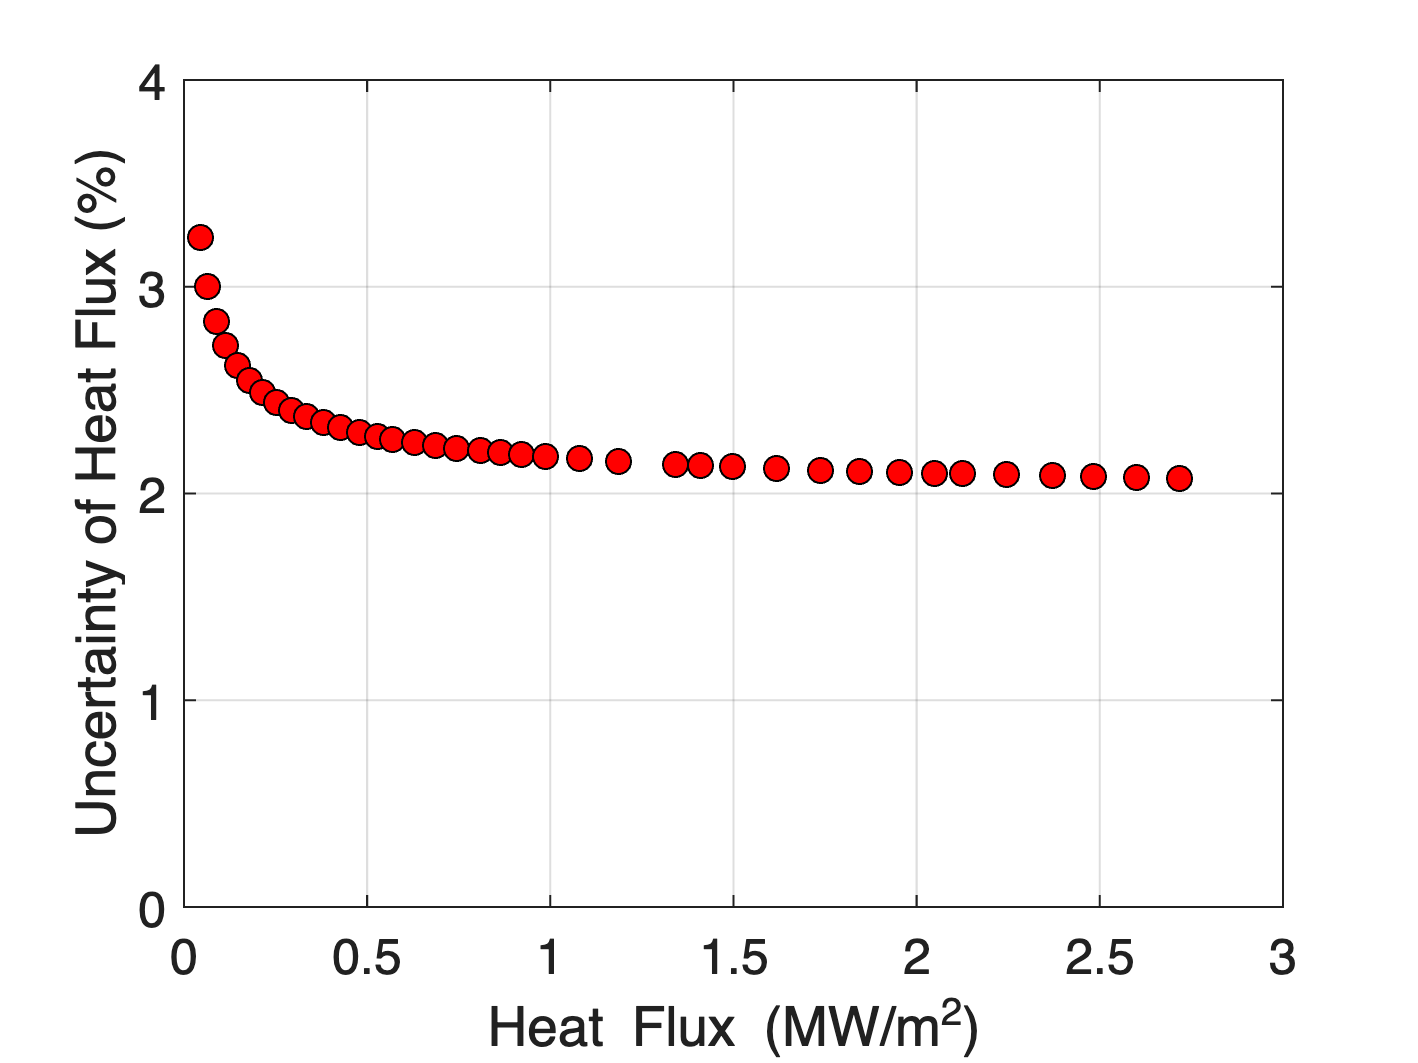
\includegraphics[width=\columnwidth]{Figure/Fig11_HeatFluxUncertainty.png}}
\caption{Relative uncertainty of the wall heat flux, $\delta q''/q''$.}
\label{fig:fig11}
\end{figure}

\begin{figure}[htbp]
\centerline{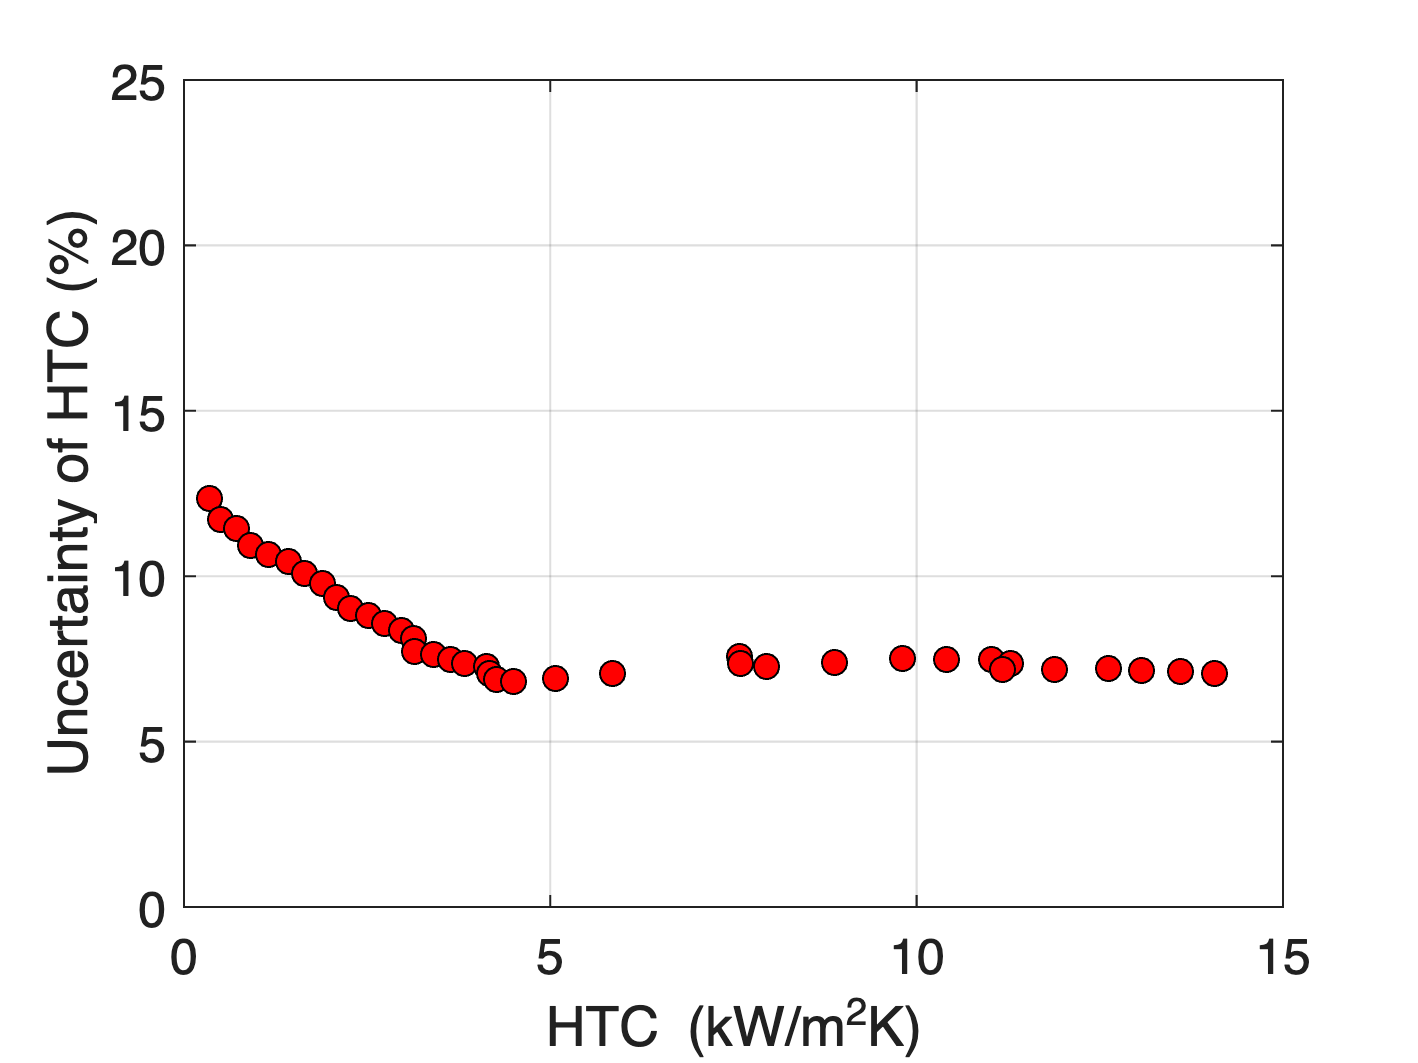
\includegraphics[width=\columnwidth]{Figure/Fig12_HTCUncertainty.png}}
\caption{Relative uncertainty of the heat transfer coefficient, $\delta h/h$.}
\label{fig:fig12}
\end{figure}

Taken together, Figs.~\ref{fig:fig04}--\ref{fig:fig12} demonstrate that the wire temperature derived from resistance thermometry is the dominant source of uncertainty in the final heat transfer coefficient. The direct voltage and current measurements alone would yield sub-2\% accuracy on power and heat flux, but the resistivity-based estimate of $T_{\mathrm{wire}}$ inflates the uncertainty of the wall superheat $\Delta T = T_{\mathrm{wire}} - T_{\mathrm{water}}$ to $\pm 15$--$20~^{\circ}\mathrm{C}$ at the highest temperatures. This insight informs both the interpretation of the boiling curve presented next and the suggestions for improved instrumentation in the conclusion.

% ============================================================
\section{Results and Discussion}
\label{sec:results}
% ============================================================

\subsection{Boiling Curves}
The defining outcome of the experiment is the family of boiling curves shown in Figs.~\ref{fig:fig13}--\ref{fig:fig15}, which plot, respectively, the heating power, the heat flux, and the heat transfer coefficient against the wire (or wall) temperature, with the propagated uncertainties displayed as error bars in both directions. All three plots reveal the same qualitative structure: a smooth ``natural-convection'' branch in which the heat input increases gradually with wire temperature, followed by a sharp transition into a second branch in which much higher power is dissipated while the wire temperature actually decreases.

\begin{figure}[htbp]
\centerline{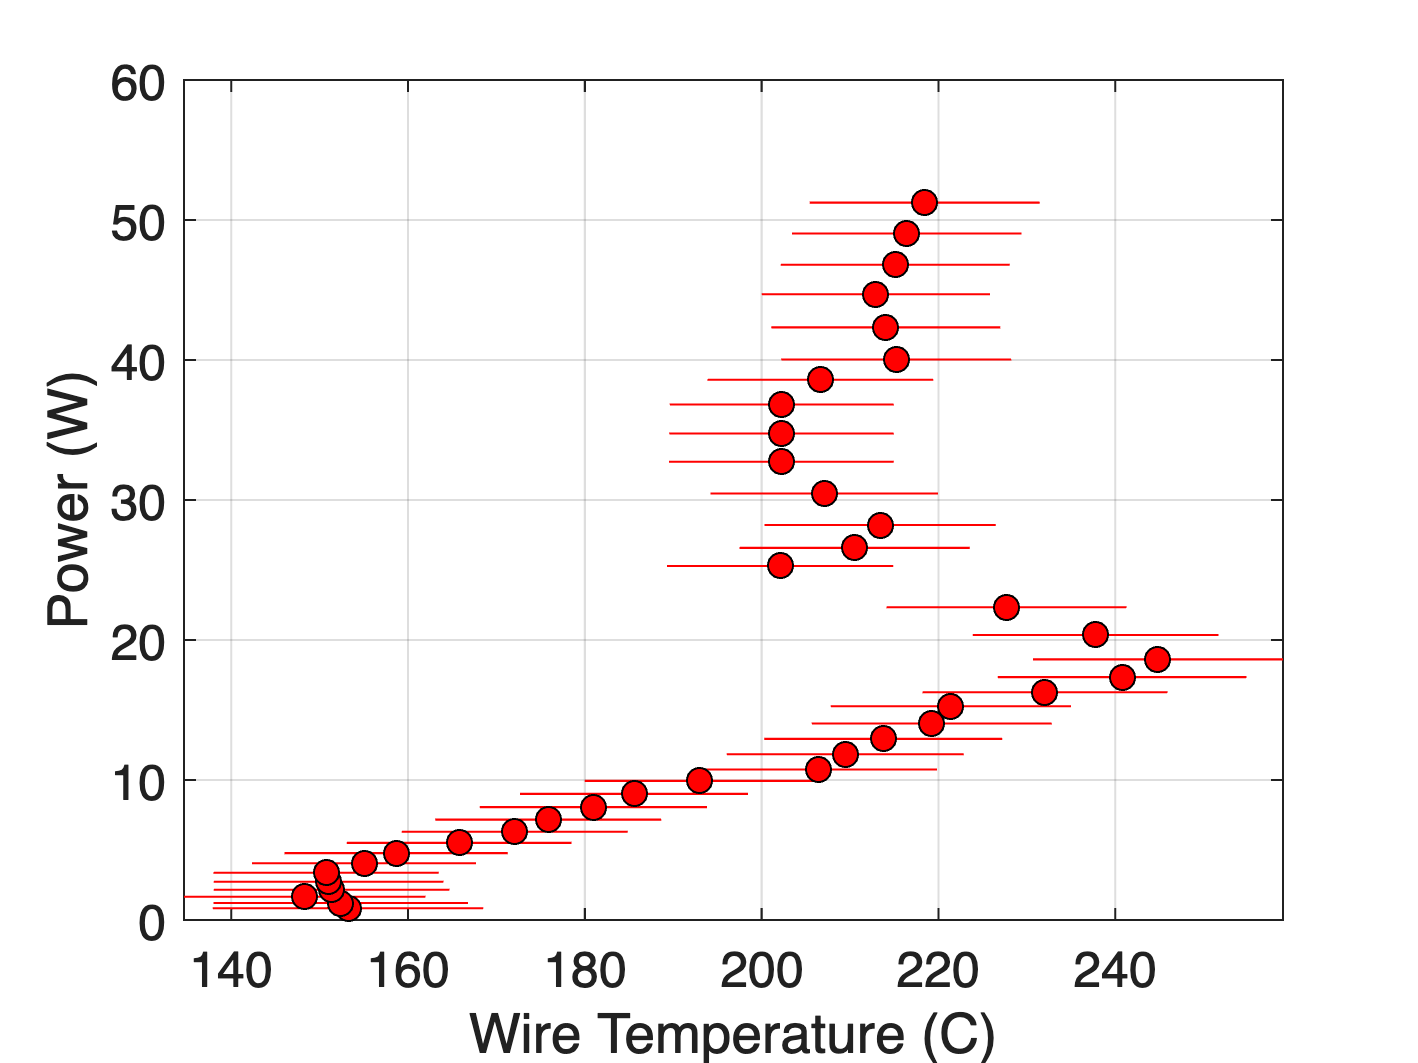
\includegraphics[width=\columnwidth]{Figure/Fig13_BoilingCurve_Power.png}}
\caption{Boiling curve in $(T_{\mathrm{wire}},W)$ coordinates. Error bars indicate the RSS-propagated uncertainties from \eqref{eq:rho}--\eqref{eq:HTC}.}
\label{fig:fig13}
\end{figure}

\begin{figure}[htbp]
\centerline{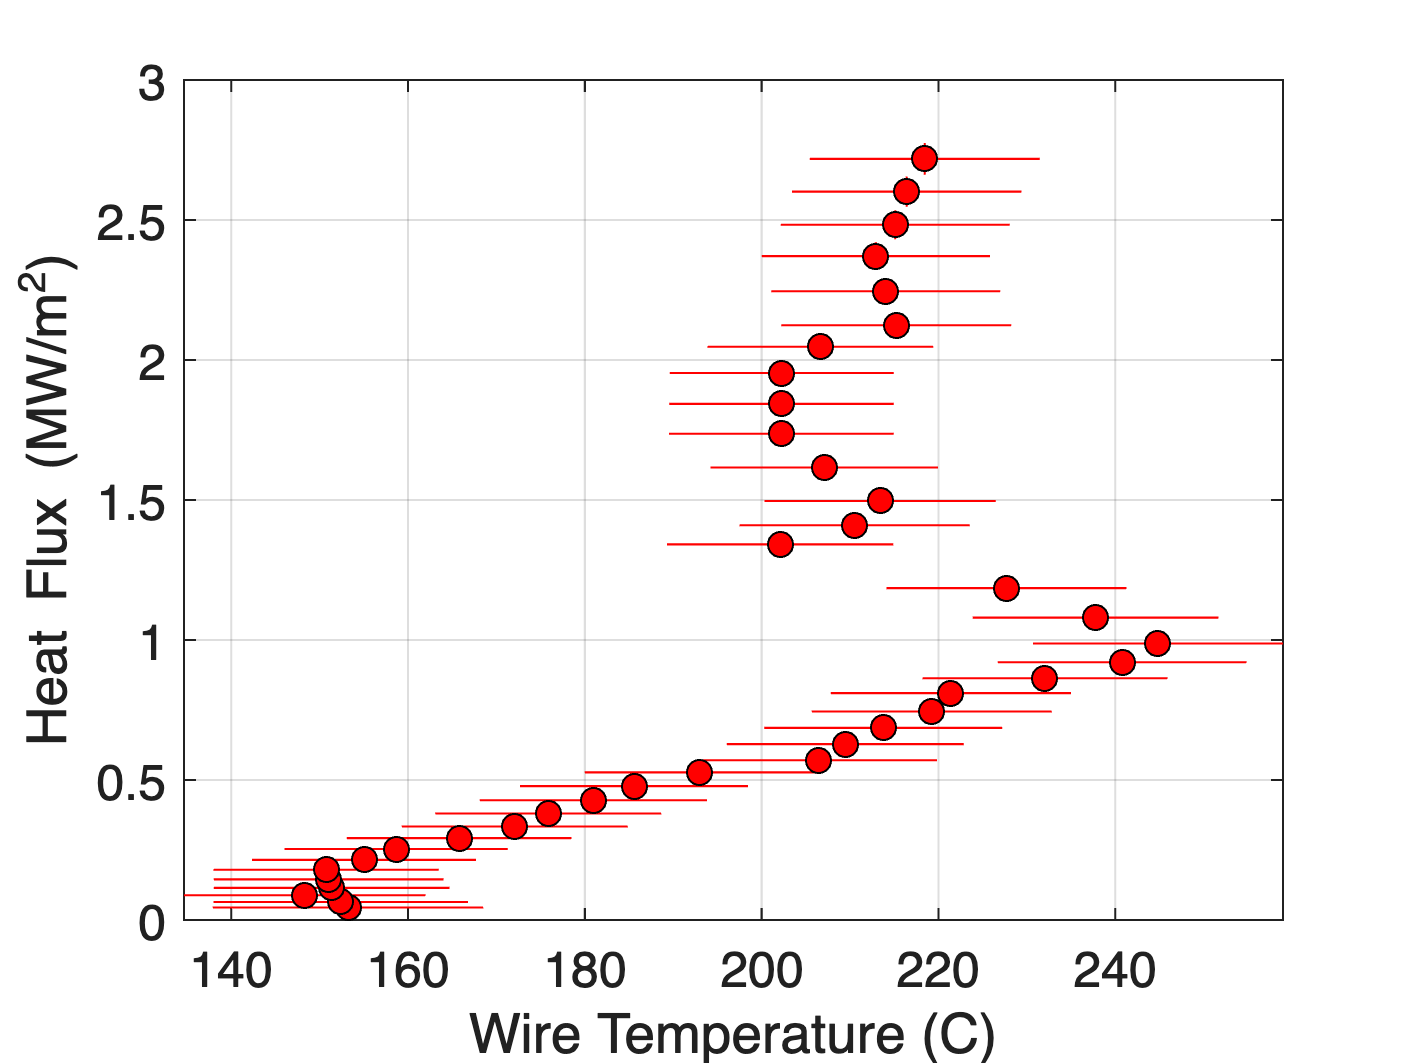
\includegraphics[width=\columnwidth]{Figure/Fig14_BoilingCurve_HeatFlux.png}}
\caption{Boiling curve in $(T_{\mathrm{wire}},q'')$ coordinates. The peak heat flux reached in this experiment is $q''_{\max}\approx 2.7~\mathrm{MW/m^2}$, of the same order as Nukiyama's reported $Q_{\max}$.}
\label{fig:fig14}
\end{figure}

\begin{figure}[htbp]
\centerline{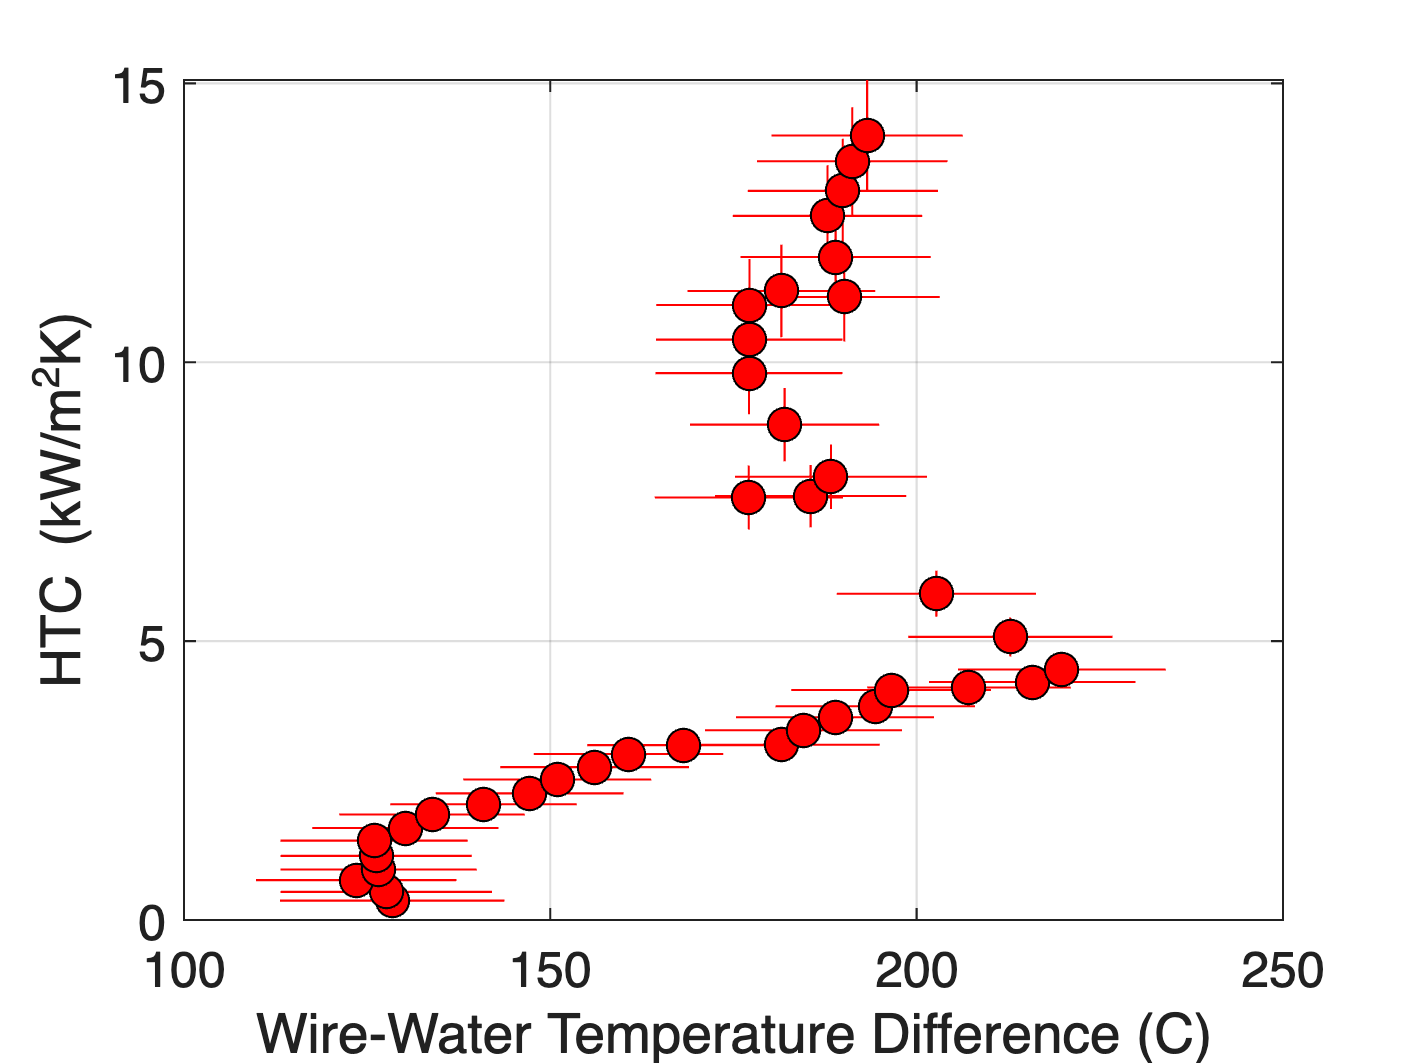
\includegraphics[width=\columnwidth]{Figure/Fig15_BoilingCurve_HTC.png}}
\caption{Heat transfer coefficient $h$ as a function of the wire-water temperature difference $\Delta T = T_{\mathrm{wire}}-T_{\mathrm{water}}$. The jump from $\sim 5$ to $\sim 11~\mathrm{kW/(m^2\,K)}$ near $\Delta T \approx 175$--$180~^{\circ}\mathrm{C}$ marks the onset of nucleate boiling.}
\label{fig:fig15}
\end{figure}

\begin{figure}[htbp]
\centerline{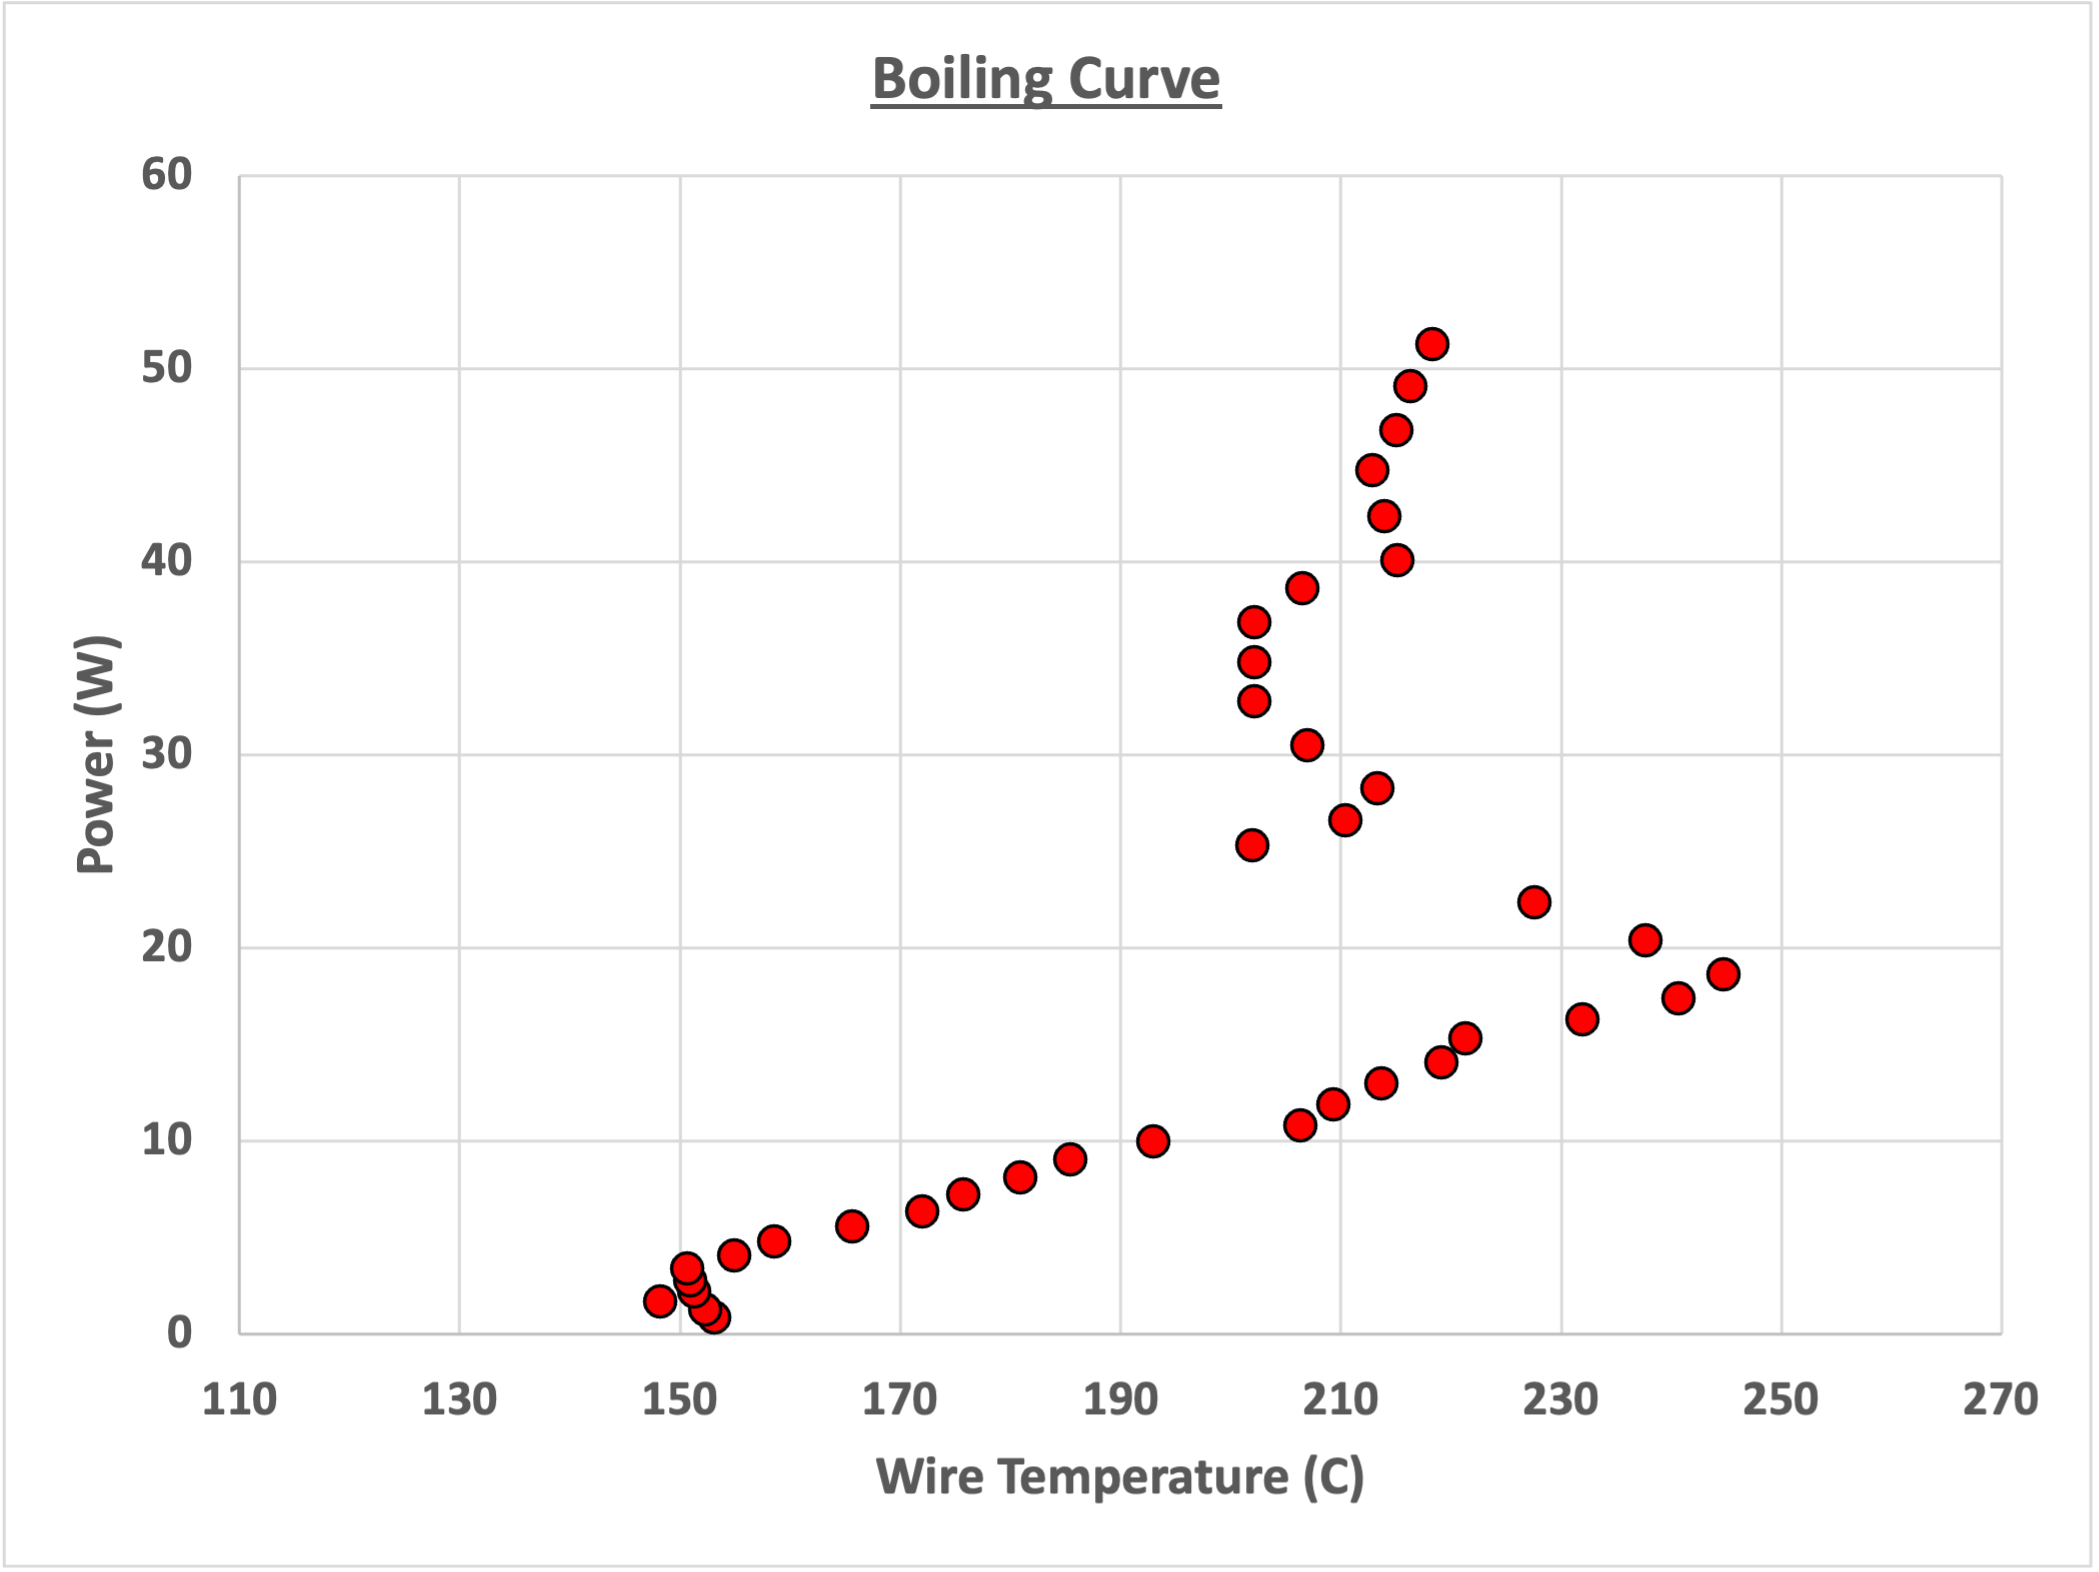
\includegraphics[width=\columnwidth]{Figure/power_vs_Twire.png}}
\caption{Same data as Fig.~\ref{fig:fig13}, replotted from the raw spreadsheet for clarity of the regime structure.}
\label{fig:fig_extra}
\end{figure}

\subsection{Identification of the Boiling Regimes}
On the lower branch the wire temperature rises continuously from $\approx 150~^{\circ}\mathrm{C}$ at $W\approx 1~\mathrm{W}$ to $\approx 244~^{\circ}\mathrm{C}$ near $W\approx 17~\mathrm{W}$. The corresponding HTC (Fig.~\ref{fig:fig15}) increases gradually from below $1~\mathrm{kW/(m^2\,K)}$ to roughly $5~\mathrm{kW/(m^2\,K)}$. These values are consistent with single-phase natural convection enhanced by sporadic bubble nucleation: the wire is well above the saturation temperature of water, but the bulk pool remains $\approx 75~^{\circ}\mathrm{C}$ subcooled, so any bubbles that form at the wire surface condense rapidly in the surrounding liquid and do not contribute significantly to net vapor generation. Visual observation during the experiment confirmed only small, isolated bubbles attached to the wire in this regime.

Beyond the local maximum of $T_{\mathrm{wire}}$, the data abruptly migrate to a second branch on which $W$ continues to grow up to $\approx 51~\mathrm{W}$ while $T_{\mathrm{wire}}$ drops back into the $200$--$220~^{\circ}\mathrm{C}$ window. This corresponds in Fig.~\ref{fig:fig15} to an upward jump of the HTC into the $8$--$14~\mathrm{kW/(m^2\,K)}$ band. The accompanying visual observation was an immediate intensification of bubbling along the entire wire length: vapor plumes detached continuously and rose to the free surface. The physical interpretation is that, once a sufficient density of active nucleation sites has been activated, the wire enters the fully developed nucleate boiling regime, in which the latent heat carried away by departing bubbles dominates the energy balance. The associated dramatic increase of $h$ (a factor of $\sim 2$--$3$ relative to the natural-convection branch) is precisely the phenomenon that makes pool boiling attractive for high-flux thermal management.

\subsection{Peak Heat Flux and Comparison with Nukiyama}
The maximum heat flux attained on the upper branch is $q''_{\max}\approx 2.7~\mathrm{MW/m^2}$ (Fig.~\ref{fig:fig14}). Translated to Nukiyama's units this is $\approx 2.3\times 10^{6}~\mathrm{kcal/(m^2\,h)}$, somewhat above the value $1.08$--$1.80\times 10^{6}~\mathrm{kcal/(m^2\,h)}$ originally reported by Nukiyama for saturated water on a $0.14~\mathrm{mm}$ platinum wire~\cite{nukiyama1966}. Two factors plausibly explain the higher peak observed here. First, the strong subcooling of the bulk pool ($\Delta T_{\mathrm{sub}} \approx 75~^{\circ}\mathrm{C}$) is known to enhance the critical heat flux substantially, because cold liquid sweeping in from the bulk reduces the residence time of vapor on the wire surface and delays film formation. Second, the wire used in the present experiment is thinner ($D_w = 100~\mathrm{\mu m}$) than Nukiyama's reference case ($140~\mathrm{\mu m}$), and Nukiyama himself documented that $Q_{\max}$ increases as the diameter is reduced. Both effects point in the same direction and account, at least qualitatively, for the discrepancy.

It is important to emphasize that the experiment was terminated before the wire entered the transition or film-boiling regimes, both for instrumentation reasons (the power supply was operating near its compliance limit) and to avoid burnout of the test piece. Consequently the descending portion of the Nukiyama curve between $Q_{\max}$ and $Q_{\min}$ was not mapped. The data nevertheless reproduce the most important diagnostic feature of the curve---the abrupt jump in slope at the onset of nucleate boiling---and the magnitudes of $q''_{\max}$ and the peak HTC are within the range expected for thin-wire boiling of water.

\subsection{Role of Uncertainty}
The error bars in Figs.~\ref{fig:fig13}--\ref{fig:fig15} convey two important messages. First, the horizontal uncertainty bars on $T_{\mathrm{wire}}$ ($\pm 10$--$20~^{\circ}\mathrm{C}$) are large compared with the vertical bars on $W$ or $q''$, confirming that wire-temperature uncertainty is the dominant contributor to the overall error budget. Despite this, the gap between the two branches in Fig.~\ref{fig:fig13} ($\Delta T_{\mathrm{wire}}\approx 30~^{\circ}\mathrm{C}$ at fixed power, or $\Delta W \approx 30~\mathrm{W}$ at fixed temperature) is several times the propagated uncertainty, so the regime transition is statistically significant. Second, the HTC uncertainty in Fig.~\ref{fig:fig15} is largest at the smallest $\Delta T$, as anticipated, but the qualitative jump of $h$ at the onset of nucleate boiling lies far outside any plausible error envelope. Hence the central conclusions of the experiment---existence of a regime transition and large enhancement of $h$ in nucleate boiling---are robust to the measurement uncertainties identified in Section~\ref{sec:dp}.

\subsection{Limitations and Suggested Improvements}
Three principal limitations of the present setup are worth noting. (i)~The dominant uncertainty originates from the conversion of $\rho$ to $T_{\mathrm{wire}}$ via the shallow platinum coefficient $\alpha$. A direct, calibrated four-wire measurement of $R$ at multiple known reference temperatures, or substitution of a higher-coefficient material (e.g., nickel), would significantly tighten $\delta T_{\mathrm{wire}}$. (ii)~The wire was operated in strongly subcooled water; while this enabled an unusually high $q''_{\max}$, it precluded a direct comparison with Nukiyama's saturated-water reference values. Pre-heating the pool to saturation prior to the voltage ramp would enable a more like-for-like comparison. (iii)~No effort was made to control surface contamination or oxide build-up on the wire; the scatter visible in the data (Fig.~\ref{fig:fig13}) at fixed nominal $V$ is consistent with the surface-history effects that Nukiyama himself documented in his original work.

% ============================================================
\section{Conclusion}
% ============================================================
A pedagogically scaled replication of Nukiyama's classical pool boiling experiment has been carried out using a $100~\mathrm{\mu m}$ diameter, $60~\mathrm{mm}$ long platinum wire immersed in subcooled demineralized water and Joule-heated by a DC power supply. Voltage, current, and water temperature were recorded at 38 steady-state operating points, and the wire temperature, heating power, wall heat flux, and convective heat transfer coefficient were derived from these measurements using the temperature-dependent resistivity of platinum. RSS uncertainty propagation was carried out point-by-point on every derived quantity. The principal findings are: (i)~the boiling curve exhibits the characteristic transition from a single-phase natural-convection branch ($h\sim 1$--$5~\mathrm{kW/(m^2\,K)}$) to a fully developed nucleate boiling branch ($h\sim 8$--$14~\mathrm{kW/(m^2\,K)}$); (ii)~the peak heat flux observed prior to terminating the test, $q''_{\max}\approx 2.7~\mathrm{MW/m^2}$, is of the same order as---and somewhat higher than---Nukiyama's saturated-water reference value, plausibly because of the strong bulk subcooling and the slightly smaller wire diameter used here; (iii)~the dominant source of uncertainty in the derived boiling curve is the conversion of measured resistivity to wire temperature through the shallow temperature coefficient of platinum, and reducing this uncertainty is the most impactful single improvement that could be made to the apparatus. Notwithstanding these limitations, the experiment provides a quantitative and visually compelling demonstration of the Nukiyama regime transition, and confirms the central physical claim of the 1934 paper using equipment that is accessible to an advanced undergraduate teaching laboratory.

\section*{Acknowledgment}
The authors gratefully acknowledge the Advanced Laboratory course staff at Guangdong Technion-IIT for guidance, equipment, and laboratory access during this experiment.

\begin{thebibliography}{00}
\bibitem{nukiyama1966} S. Nukiyama, ``The maximum and minimum values of the heat $Q$ transmitted from metal to boiling water under atmospheric pressure,'' \textit{Int. J. Heat Mass Transfer}, vol.~9, pp.~1419--1433, 1966. (Translated from \textit{J. Japan Soc. Mech. Engrs}, vol.~37, pp.~367--374, 1934.)
\bibitem{austin1902} L. Austin, \textit{Z. Ver. dt. Ing.}, 1902. (As cited by Nukiyama~\cite{nukiyama1966}.)
\bibitem{jakob1933} M. Jakob and W. Linke, ``\"Uber den W\"arme\"ubergang bei der Verdampfung von Fl\"ussigkeiten an senkrechten und waagerechten Fl\"achen,'' \textit{Forsch. Ing.-Wes.}, vol.~3, pp.~75--80, 1933.
\bibitem{incropera2006} F.~P. Incropera, D.~P. DeWitt, T.~L. Bergman, and A.~S. Lavine, \textit{Fundamentals of Heat and Mass Transfer}, 6th~ed. Hoboken, NJ: Wiley, 2006.
\bibitem{cioncolini2025} A. Cioncolini, ``Nukiyama's Experiment on Pool Boiling,'' in GT034057 -- Advanced Laboratory in Mechanical Engineering, Guangdong Technion-IIT, Shantou, China, Lecture~4, 2025.
\end{thebibliography}

\end{document}
